\documentclass[11.5pt, twoside, a4paper, titlepage]{report}
\usepackage{graphicx, amssymb, amsmath, mathtools, amsthm, xfrac, mathabx}
\usepackage{tikz}
\usetikzlibrary{automata, arrows, matrix}
\providecommand{\abs}[1]{\lvert#1\rvert}
\providecommand{\equ}[0]{\begin{equation*}}
\providecommand{\eequ}[0] {\end{equation*}}
\providecommand{\bb}[1]{\mathbb{#1}}
\theoremstyle{definition}
\newtheorem{mydef}{Definition}[section]
\newtheorem{rem}[mydef]{Remark}
\newtheorem{note}[mydef]{Notation}
\newtheorem{eg}[mydef]{Example}
\theoremstyle{plain}
\newtheorem{lem}[mydef]{Lemma}
\newtheorem{thm}[mydef]{Theorem}
\newtheorem{cor}[mydef]{Corollary}
\newtheorem{prop}[mydef]{Proposition}
\newtheorem*{claim}{Claim}



\begin{document}
\title{Representation of Quivers}
\author{Chanelle Lee \\Student ID: 200646370\\Supervisor: William Crawley-Boevey}
\date{\today}
\maketitle


\tableofcontents

\chapter{Introduction}

This project aims to cover interesting topics from the area of quiver representations. The first chapter will give a brief introduction to the topics in Homological Algebra needed for bulk of the report. It will cover chain complexes, exact sequences, short exact sequences, and extensions, most importantly $Ext^1$. The the second chapter will introduce quivers and look at some interesting results about path algebras before moving onto representations of quivers and their relationship with the modules of the corresponding path algebra. Next we will cover Dynkin and Euclidean diagrams before finishing with a proof of Gabriel's Theorem. The third chapter will cover Auslander-Reiten quivers.

\chapter{Homological Algebra}

%%%%%%%%%%%%%%%%%%%%%%%%%%%%%%%%%%%%%%%%%%%%%%%%%%%%%%%
%%%%%%%%%%%%%%			CHAIN COMPLEXES 		%%%%%%%%%%%%%%%%%%%%
%%%%%%%%%%%%%%%%%%%%%%%%%%%%%%%%%%%%%%%%%%%%%%%%%%%%%%%
\section{Chain Complexes}

\begin{mydef}
A \emph{chain complex} $\mathbf{C}_{\bullet}$ consists of a sequence of $\mathbb{R}$-modules $C_i$ ($i \in \mathbb{Z}$) and morphisms of the form,
\begin{equation*}
\mathbf{C}: \qquad \dots \xrightarrow{\delta_{3}} C_2 \xrightarrow{\delta_{2}} C_1 \xrightarrow{\delta_{1 }} C_0 \xrightarrow{\delta_0} C_{-1} \xrightarrow{\delta_{-1}} C_{-2} \xrightarrow{\delta_{-2}}\dots
\end{equation*}
such that $\delta_{n-1}\delta_{n}=0$ for all $n$, i.e. the composition of any two consecutive maps is zero. The maps $\delta_n$ are called the \emph{differentials} of $C$.
\end{mydef}

\begin{rem}
It is convention that the map $\delta_n$ starts at $C_n$.
\end{rem}

\begin{eg}
If we have a field $K$ then we can create the following chain complex:
\begin{equation*}
\mathbf{C}: \qquad \dots \xrightarrow{} 0 \xrightarrow{} K^2 \xrightarrow{\Bigl(\begin{smallmatrix}1&2\\ 3&0\\ 0&0 \end{smallmatrix}\Bigr)} K^3 \xrightarrow{(\begin{smallmatrix}0 & 0 &1\end{smallmatrix})} K \xrightarrow{} 0 \xrightarrow{}\dots
\end{equation*}
We can clearly see that the maps uphold the $\delta^2=0$ condition as,
\begin{equation*}
\begin{pmatrix}0 & 0 &1
\end{pmatrix}
\begin{pmatrix}
1 & 2 \\
3 & 0\\
0 & 0
\end{pmatrix}
=\begin{pmatrix}
0 & 0
\end{pmatrix}.
\end{equation*}
\end{eg}

\begin{eg} \label{Kchaineg}
If we consider the sequence, 
\equ 
\dots \xrightarrow{} 0 \xrightarrow{} K \xrightarrow{\delta_2=\big(\begin{smallmatrix} 1\\ 0 \end{smallmatrix}\big)} K^2 \xrightarrow{\delta_1=(\begin{smallmatrix}1 & 0 \end{smallmatrix})} K \xrightarrow{} 0 \xrightarrow{} \dots
\eequ
however,
\equ
\begin{pmatrix}
1 & 0
\end{pmatrix}
\begin{pmatrix*}
1\\
0
\end{pmatrix*}
= 1 \neq 0.
\eequ
Hence, $\delta_1\delta_2 \neq0$, and so the sequence is not a chain complex. However, if we change $\delta_2$ slightly we obtain the chain complex,
\equ
\mathbf{C}: \qquad \dots \xrightarrow{} 0 \xrightarrow{} K \xrightarrow{\big(\begin{smallmatrix} 1\\ 0 \end{smallmatrix}\big)} K^2 \xrightarrow{(\begin{smallmatrix}0 & 1 \end{smallmatrix})} K \xrightarrow{} 0 \xrightarrow{} \dots
\eequ
since, 
\equ
\begin{pmatrix}
1 & 0
\end{pmatrix}
\begin{pmatrix*}
0\\
1
\end{pmatrix*}
= 1 \neq 0.
\eequ
\end{eg}

\begin{mydef}
For a chain complex,
\begin{equation*}
\mathbf{C}: \qquad \dots \xrightarrow{} C_{n+1} \xrightarrow{\delta_{n+1 }} C_{n} \xrightarrow{\delta_{n}} C_{n-1} \xrightarrow{} \dots
\end{equation*}
we define:
\begin{equation*}
Z_n(\mathbf{C})=ker(\delta_n) \quad \& \quad B_n(\mathbf{C})=im(\delta_{n+1}).
\end{equation*}
\end{mydef}

To explore the relationship between $Z_n(\mathbf{C})$ and $B_n(\mathbf{C})$, the following is a solution to Exercise 2.14 in \cite{Rotman}.(Note the example will not be provided here as exactness has not yet been covered.)

\begin{lem}\label{iminkerlem}
Let,
\begin{equation*}
A \xrightarrow{f} B \xrightarrow{g} C,
\end{equation*}
be a sequence of module maps. Then $gf=0$ if and only if $im(f)\subseteq im(g)$.
\end{lem}
\begin{proof}
Suppose $gf=0$, i.e., for all $a\in A$, $g(f(a))=0$ which implies that $f(a)\in ker(g)$ for all $a \in A$. Hence, $im(f) \subseteq ker(g)$.\\
Conversely, suppose that $im(f) \subseteq ker(g)$. Every element $b\in im(f)$ is also an element of $ker(g)$, thus $gf=0$.
\end{proof}

\begin{mydef} \label{homologydefn}
If $\mathbf{C}$ is a chain complex then its \emph{homology} is defined to be,
\begin{equation*}
H_n(\mathbf{C})=\frac{ker(\delta_n:C_n \rightarrow C_{n-1})}{im(\delta_{n+1}:C_{n+1} \rightarrow C_n)}=\frac{Z_n(\mathbf{C})}{B_n(\mathbf{C})},
\end{equation*}
which is an $\bb{R}$-module.
\end{mydef}


The subsequent proposition is the solution to Exercise 6.1 in \cite{Rotman}.

\begin{prop}
If $\mathbf{C}$ is a chain complex with $C_n=0$ for some $n$ then $H_n(\mathbf{C})=0$.
\end{prop}
\begin{proof}
Well suppose we have such a chain complex, 
\equ
\mathbf{C}: \qquad \dots \xrightarrow{} C_{n+1} \xrightarrow{\delta_{n+1}} 0 \xrightarrow{\delta_n} C_{n-1} \xrightarrow{} \dots
\eequ
the the homology is,
\equ
H_n(\mathbf{C})=\frac{ker(\delta_n: 0 \to C_{n-1}}{im(\delta_{n+1}: C_{n+1}\to 0)},
\eequ
as the only element in $C_n$ is the zero element, and so, $H_n(\mathbf{C})=0$, as required.\\
\end{proof}

Examples \ref{chainMeg} and \ref{chainZeg} are taken from \cite{CB1} and are included here because they are felt to be the clearest at demonstrating a chain complex and homology, however, the more general statement of the second example is presented as Proposition \ref{chainhomprop} because it is an interesting result.

\begin{eg}
 \label{chainMeg}
 If we take a module $M$ then we can make a chain complex;
\begin{equation*}
\mathbf{C}: \qquad \dots \xrightarrow{} 0 \xrightarrow{} M \xrightarrow{} 0 \xrightarrow{} \dots
\end{equation*}
where $M$ is at degree $n$. Then the homology will be:
\begin{equation*}
H_i(\mathbf{C})=\begin{cases}
\frac{ker(M \rightarrow 0)}{im(0 \rightarrow M)}=M & i=n,\\
0 & \text{otherwise}.
\end{cases}
\end{equation*}
\end{eg}

\begin{prop}  \label{chainhomprop}
If we have a module homomorphism between $R$-modules, $f: M \xrightarrow{} N$, the we get the chain complex,
\equ
\mathbf{C}: \qquad \underset{\text{deg}}{\dots} \xrightarrow{}\underset{n+2}{0} \xrightarrow{} \underset{n+1}{M} \xrightarrow{f}\underset{n}{N} \xrightarrow{} \underset{n-1}{0} \xrightarrow{}\dots ,
\eequ
and the homology becomes,
\equ
H_i(\mathbf{C})=
\begin{cases}
\frac{N}{im(f)}=coker(f) & i=n\\
ker(f) & i=n+1\\
0 & \text{otherwise}.
\end{cases}
\eequ
\end{prop}
\begin{proof}
Firstly, at degree $n$ we have that,
\equ
H_n(\mathbf{C})=\frac{ker(N\xrightarrow{}0)}{im(M\xrightarrow{f}N)}=\frac{N}{im(f)}=coker(f).
\eequ
Then at degree $n+1$ we have that,
\equ
H_{n+1}(\mathbf{C})=\frac{ker(M\xrightarrow{f}N)}{im(0\xrightarrow{}M)}=ker(f).
\eequ
Finally, it is clear that everywhere else there is no homology.
\end{proof}

\begin{note}
Here, 
\equ
Coker(f)= \frac{\text{Codomain of }f}{\text{Image of }f},
\eequ
is the \emph{cokernel} of the map $f$.
\end{note}

\begin{eg} \label{chainZeg}
We can have a chain complex of $\mathbb{Z}$-modules,
\equ
\mathbf{C}: \qquad \underset{\text{deg}}{\dots} \xrightarrow{}\underset{2}{0} \xrightarrow{} \underset{1}{\mathbb{Z}} \xrightarrow{a}\underset{0}{\mathbb{Z}} \xrightarrow{} \underset{-1}{0} \xrightarrow{}\dots 
\eequ
where the map $a$ is right multiplication by some $a \in \mathbb{Z}$. The homology is,
\equ
H_i(\mathbf{C}) = 
\begin{cases}
\frac{ker(\mathbb{Z}\xrightarrow{} 0)}{im(\mathbb{Z}\xrightarrow{a}\mathbb{Z})}=\frac{\mathbb{Z}}{a\mathbb{Z}} & i=0,\\
0 & \text{otherwise}.
\end{cases}
\eequ
Note that,
\equ
H_0(C)=\frac{\bb{Z}}{a\bb{Z}}= \frac{\text{Codomain of }f}{\text{Image of }f}=coker(a).
\eequ
Also,
\equ
H_1(C)=\frac{ker(\bb{Z}\xrightarrow{a}\bb{Z})}{im(0\xrightarrow{}\bb{Z})}=ker(a)=0,
\eequ
because $ker(a)$ is empty.
\end{eg}

\begin{mydef}
\begin{itemize}
\item The elements of $B_n(\mathbf{C})$ are called \emph{$n-$boundaries}.
\item The elements of $Z_n(\mathbf{C})$ are called \emph{$n-$cycles}.
\end{itemize}
\end{mydef}

\begin{rem} %Will we use this notation??
If $x\in Z_n(\mathbf{C})$ then its image in $H_n(\mathbf{C})$ is usually written as $[x]$.
\end{rem}

\begin{mydef}
A chain complex $\mathbf{C}$ is said to be:
\begin{itemize}
\item \emph{acyclic} if $H_n(\mathbf{C})=0$ for all $n$.
\item \emph{bounded above} if there exists some $n\in \mathbb{N}$, $C_k=0$ for all $k>n$.
\item \emph{bounded below} if for some $n \in \mathbb{N}$, $C_k=0$ for all $k<n$.
\item \emph{bounded} if it is bounded above and below.
\item \emph{non-negative}  if $C_n=0$ for $n<0$.
\end{itemize}
\end{mydef}

\begin{eg}
All the chain complexes in the previous examples are bounded both above and below, however, neither is acyclic as they both have instances where the homology is non-zero. The chain complex in Example \ref{chainZeg} is non-negative because $C_n\neq 0$ only when $n=0,1$.
\end{eg}

\begin{eg}
If we take another look at the chain complex in Example \ref{Kchaineg},
\equ
\mathbf{C}: \qquad \underset{\text{deg}}{\dots} \xrightarrow{} 0 \xrightarrow{} \underset{1}{K} \xrightarrow{\big(\begin{smallmatrix} 1\\ 0 \end{smallmatrix}\big)} \underset{0}{K^2} \xrightarrow{(\begin{smallmatrix}0 & 1 \end{smallmatrix})}\underset{-1}{K} \xrightarrow{} 0 \xrightarrow{} \dots
\eequ
the homologies are, 
\begin{align*}
H_1(\mathbf{C}) &=\frac{ker(K\xrightarrow{\big(\begin{smallmatrix} 1\\ 0 \end{smallmatrix}\big)}K^2)}{im(0 \xrightarrow{}K)}\cong \frac{K}{K} \cong 0,\\
H_0(\mathbf{C}) &=\frac{ker(K^2\xrightarrow{(\begin{smallmatrix} 1 & 0 \end{smallmatrix})}K)}{im(K\xrightarrow{\big(\begin{smallmatrix} 1\\ 0 \end{smallmatrix}\big)}K^2)}\cong \frac{K}{K} \cong 0,\\
H_{-1}(\mathbf{C}) &=\frac{ker(K\xrightarrow{}0)}{im(K^2\xrightarrow{(\begin{smallmatrix} 1 & 0 \end{smallmatrix})}K))}\cong \frac{K}{K} \cong 0.\\
\end{align*}
Thus $H_n(\mathbf{C})=0$ for all $n$ and so $\mathbf{C}$ is an acyclic chain complex. Later in the report, we will see that $\mathbf{C}$ is in fact a short exact sequence.
\end{eg}

\begin{eg}
The chain complex,
\equ
\mathbf{C}: \qquad \underset{\text{deg}}{\underset{}{\dots}} \xrightarrow{3}\underset{1}{\frac{\bb{Z}}{9\bb{Z}}} \xrightarrow{3}\underset{0}{\frac{\bb{Z}}{9\bb{Z}}} \xrightarrow{3}\underset{-1}{\frac{\bb{Z}}{9\bb{Z}}} \xrightarrow{} \dots
\eequ
where the differentials are the maps,
\equ
\delta_n:\frac{\bb{Z}}{9\bb{Z}}\xrightarrow{}\frac{\bb{Z}}{9\bb{Z}}\text{, } z+9\bb{Z}\mapsto 3z+9\bb{Z},
\eequ
is unbounded. It is also acyclic, since the homology is,
\equ
H_n(\mathbf{C})=\frac{ker(\delta_n:\frac{\bb{Z}}{9\bb{Z}}\xrightarrow{}\frac{\bb{Z}}{9\bb{Z}})}{im(\delta_n:\frac{\bb{Z}}{9\bb{Z}}\xrightarrow{}\frac{\bb{Z}}{9\bb{Z}})}\cong \frac{\bb{Z}/3\bb{Z}}{\bb{Z}/3\bb{Z}} \cong 0, 
\eequ
for all $n$.
\end{eg}

\begin{mydef}
A \emph{cochain complex} $\mathbf{C}^{\bullet}$ consists of a sequence of $\mathbb{R}$-modules $C^i$ ($i \in \mathbb{Z}$) and morphisms of the form,
\begin{equation*}
\mathbf{C}: \qquad \dots \xrightarrow{\delta^{-3}} C^{-2} \xrightarrow{\delta^{-2}} C^{-1} \xrightarrow{\delta^{-1 }} C^0 \xrightarrow{\delta^0} C^{1} \xrightarrow{\delta^{1}} C^{2} \xrightarrow{\delta^{2}} \dots
\end{equation*}
such that $\delta^{n-1}\delta^{n}=0$ for all $n$, i.e. the composition of any two consecutive maps is zero.
\end{mydef}

\begin{rem}
Chain and cochain complexes can be thought of as almost identical constructs with the only difference being thenumbering of the chain. The degree of a chain complex \emph{decreases} from left to right, whereas, the degree of a cochain complex \emph{increses} from left to right. So, we can compute one from the other by setting $C^{-n}=C_n$, or equivalently $C^n=C_{-n}$; this is called \emph{renumbering}.
\end{rem}

\begin{mydef}
If $\mathbf{C}$ is a cochain complex then its \emph{cohomology} is defined to be,
\begin{equation*}
H^n(\mathbf{C})=\frac{ker(\delta^n:C^n \rightarrow C^{n+1})}{im(\delta^{n-1}:C^{n-1} \rightarrow C^n)} =\frac{Z^n(\mathbf{C})}{B^n(\mathbf{C})}.
\end{equation*}
\begin{itemize}
\item The elements of $B_n(\mathbf{C})$ are called \emph{$n-$coboundaries}.
\item The elements of $Z_n(\mathbf{C})$ are called \emph{$n-$cocycles}.
\end{itemize}
\end{mydef}

\begin{eg}
We can renumber the chain complex in Example \ref{chainZeg} to get the cochain complex, 
\equ
\mathbf{C}: \qquad \underset{\text{deg}}{\dots} \xrightarrow{}\underset{-2}{0} \xrightarrow{} \underset{-1}{\mathbb{Z}} \xrightarrow{a}\underset{0}{\mathbb{Z}} \xrightarrow{} \underset{1}{0} \xrightarrow{}\dots 
\eequ
Its cohomology is,
\equ
H^i(\mathbf{C}) = 
\begin{cases}
\frac{ker(\mathbb{Z}\xrightarrow{} 0)}{im(\mathbb{Z}\xrightarrow{a}\mathbb{Z})}=\frac{\mathbb{Z}}{a\mathbb{Z}} & i=0,\\
0 & \text{otherwise}.
\end{cases}
\eequ
\end{eg}

\begin{mydef}
Let $\mathbf{C}$ be a chain complex of left $R$-modules. If M is a left $R$-module then \emph{$Hom(\mathbf{C}, M)$} is the cochain complex where,
\equ
Hom(\mathbf{C}, M)^n=Hom(C_n, M),
\eequ
and the differentials, 
\equ
\delta^n: Hom(\mathbf{C}, M)^n \to Hom(C, M)^{n+1},
\eequ
are induced by the differentials of $\mathbf{C}$, $\delta_n:C_{n+1}\to C_n$. The cohomology of this cochain complex is denoted $H^n(\mathbf{C}, M)$.
\end{mydef}

The following example is a generalised version of one found in \cite{CB1}.

\begin{eg}
Consider the acyclic chain complex, 
\equ
\mathbf{C}: \qquad \underset{\text{deg}}{\underset{}{\dots}} \xrightarrow{}0 \xrightarrow{} \underset{1}{\underset{}{\bb{Z}}} \xrightarrow{n} \underset{0}{\underset{}{\bb{Z}}} \xrightarrow{nat} \underset{-1}{\frac{\bb{Z}}{n\bb{Z}}} \xrightarrow{} \dots
\eequ
So applying $Hom(-, \bb{Z})$ we gives the cochain complex, 
\equ
\mathbf{C'}: \qquad \underset{\text{deg}}{\underset{}{\dots}} \xrightarrow{}0 \xrightarrow{} \underset{1}{\underset{}{\bb{Z}}} \xrightarrow{n} \underset{0}{\underset{}{\bb{Z}}} \xrightarrow{nat} \underset{-1}{\frac{\bb{Z}}{n\bb{Z}}} \xrightarrow{} \dots
\eequ
which has cohomology,
\equ
H^i(\mathbf{C'}, \bb{Z})=
\begin{cases}
\frac{ker(\bb{Z}\to0)}{im(\bb{Z}\xrightarrow{n}\bb{Z})} \cong \frac{\bb{Z}}{n\bb{Z}} & i=0, \\
0 & \text{otherwise.}
\end{cases}
\eequ
Notice that despite the chain complex being acyclic, its cohomology induced by $Hom(-, \bb{Z})$  is not zero everywhere.
\end{eg}

\begin{mydef}
A \emph{chain map}  $f: \mathbf{C} \to \mathbf{D}$, with $\mathbf{C}$ and $\mathbf{D}$ chain complexes, is given by a homomorphism $f_n: \mathbf{C}_n \to \mathbf{D}_n$ for each $n$, such that each square in the following diagram commutes, 
\equ
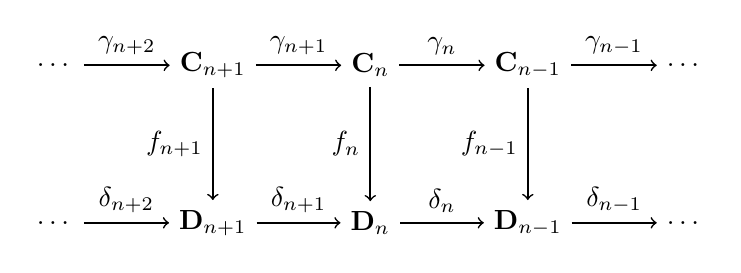
\begin{tikzpicture}[->,-latex, auto, every path/.style={->, semithick}, main node/.style={}]
\node	[main node]		(1) at (0,0)		{\dots};
\node	[main node]		(2) at (2,0)		{$\mathbf{C}_{n+1}$};
\node	[main node]		(3) at (4,0)		{$\mathbf{C}_{n}$};
\node [main node]		(4) at (6,0)		{$\mathbf{C}_{n-1}$};
\node [main node]		(5) at (8,0)		{$\dots$};
\node	[main node]		(6) at (0,-2)		{\dots};
\node	[main node]		(7) at (2,-2)		{$\mathbf{D}_{n+1}$};
\node	[main node]		(8) at (4,-2)		{$\mathbf{D}_{n}$};
\node [main node]		(9) at (6,-2)		{$\mathbf{D}_{n-1}$};
\node [main node]		(10) at (8,-2)		{\dots};

\draw (1) edge node [auto] {$\gamma_{n+2}$} (2);
\draw (2) edge node [auto] {$\gamma_{n+1}$} (3);
\draw (3) edge node [auto] {$\gamma_n$} (4);
\draw (4) edge node [auto] {$\gamma_{n-1}$} (5);
\draw (6) edge node [auto] {$\delta_{n+2}$} (7);
\draw (7) edge node [auto] {$\delta_{n+1}$} (8);
\draw (8) edge node [auto] {$\delta_n$} (9);
\draw (9) edge node [auto] {$\delta_{n-1}$} (10);
\draw (2) edge node [auto, swap] {$f_{n+1}$} (7);
\draw (3) edge node [auto, swap] {$f_n$} (8);
\draw (4) edge node [auto, swap] {$f_{n-1}$} (9);
\end{tikzpicture}
\eequ
Note that there is an equivalent notion of a \emph{cochain map} of cochain complexes.
\end{mydef}

\begin{eg}
If we have the following diagram,
\equ
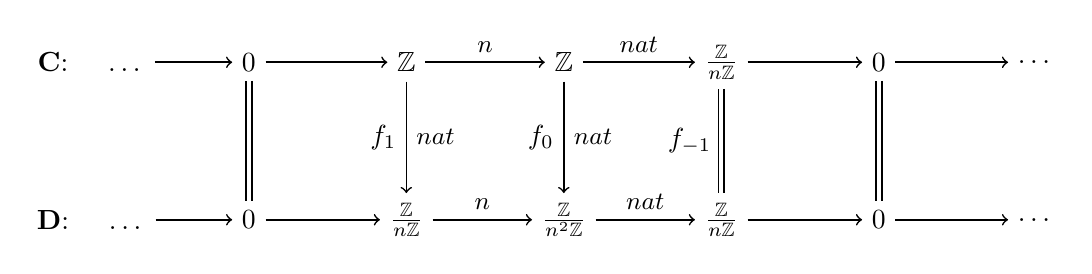
\begin{tikzpicture}[->,-latex, auto, main path/.style={->, semithick}, main node/.style={}]
\node	[main node]		(1) at (0,0)		{$\mathbf{C}$: \quad \dots};
\node	[main node]		(2) at (2,0)		{$0$};
\node	[main node]		(3) at (4,0)		{$\bb{Z}$};
\node [main node]		(4) at (6,0)		{$\bb{Z}$};
\node [main node]		(5) at (8,0)		{$\frac{\bb{Z}}{n\bb{Z}}$};
\node	[main node]		(11) at (10,0)	{$0$};
\node [main node] 		(12) at (12,0)	{\dots};
\node	[main node]		(6) at (0,-2)		{$\mathbf{D}$: \quad \dots};
\node	[main node]		(7) at (2,-2)		{$0$};
\node	[main node]		(8) at (4,-2)		{$\frac{\bb{Z}}{n\bb{Z}}$};
\node [main node]		(9) at (6,-2)		{$\frac{\bb{Z}}{n^2\bb{Z}}$};
\node [main node]		(10) at (8,-2)	{$\frac{\bb{Z}}{n\bb{Z}}$};
\node [main node]		(13) at (10,-2)	{$0$};
\node [main node]		(14) at (12,-2)	{\dots};

\draw (1) edge [main path] node [auto] {$$} (2);
\draw (2) edge [main path] node [auto] {$$} (3);
\draw (3) edge [main path] node [auto] {\small $n$} (4);
\draw (4) edge [main path] node [auto] {\small $nat$} (5);
\draw (5) edge [main path] (11);
\draw (11) edge [main path] (12);
\draw (6) edge [main path] node [auto] {$$} (7);
\draw (7) edge [main path] node [auto] {$$} (8);
\draw (8) edge [main path] node [auto] {\small $n$} (9);
\draw (9) edge [main path] node [auto] {\small $nat$} (10);
\draw (10) edge [main path] (13);
\draw (13) edge [main path] (14);
\draw (3) edge [main path] node [auto, swap] {$f_{1}$} node [auto] {\small $nat$} (8);
\draw (4) edge [main path] node [auto, swap] {$f_{0}$} node [auto] {\small $nat$} (9);
\draw (5) edge [-, semithick, double, double distance=1.5pt] node [auto, swap] {$f_{-1}$} (10);
\draw (11) edge [-, semithick, double, double distance=1.5pt] (13);
\draw (2) edge [-, semithick, double, double distance=1.5pt] (7);
\end{tikzpicture}
\eequ
then we can see that our non trivial chain maps are, 
\begin{align*}
f_{1} &: \bb{Z} \to \frac{\bb{Z}}{n\bb{Z}}, \quad z \mapsto z+n\bb{Z},\\
f_0 &: \bb{Z} \to \frac{\bb{Z}}{n^2\bb{Z}}, \quad z \mapsto z+n^2\bb{Z}, \\
f_{1} &: \frac{\bb{Z}}{n\bb{Z}} \to \frac{\bb{Z}}{n\bb{Z}}, \quad z+n\bb{Z} \mapsto z+n\bb{Z}, 
\end{align*}
and they satisfy, 
\equ
f_0(\gamma_1(z))=f_0(nz)=nz+n\bb{Z}=0\quad \& \quad \delta_1(f_1(z))=\delta_1(z+n\bb{Z})=nz+n\bb{Z}=0.
\eequ
Simmilarly, we can see that the other chain maps make the diagram commute.
\end{eg}





















%%%%%%%%%%%%%%%%%%%%%%%%%%%%%%%%%%%%%%%%%%%%%%%%%%%%%
%%%%%%%%%%%%%%%%		EXACT SEQUENCES			%%%%%%%%%%%%%%%%%%%%
%%%%%%%%%%%%%%%%%%%%%%%%%%%%%%%%%%%%%%%%%%%%%%%%%%%%%

\section{Exact Sequences}

\begin{mydef}
A finite or infinite sequence of $R$-morphisms and left $R$-modules,
\begin{equation*}
\dots \xrightarrow{} L \xrightarrow{f}M \xrightarrow{g} N \xrightarrow{} \dots
\end{equation*}
is said to be \emph{exact} at $M$ if $imf=kerg$. A finite or infinite sequence of $R$-morphisms and left $R$-modules,
\begin{equation*}
\dots \xrightarrow{f_{n+2}} M_{n+1} \xrightarrow{f_{n+1}} M_n \xrightarrow{f_n} M_{n-1} \xrightarrow{f_{n-1}} \dots
\end{equation*}
is said to be an \emph{exact sequence} if it is exact at every $M_i$, i.e. $imf_i=kerf_{i+1}$. 
\end{mydef}

\begin{eg}
The finite sequence,
\begin{equation*}
0\xrightarrow{}K\xrightarrow{f}K^2\xrightarrow{g}K^2\xrightarrow{h}K^2\xrightarrow{}0,
\end{equation*}
where $f(x)=(x,0)$, $g(x, y)=(0,y)$, and $h(x,y)=(x,0)$ is an exact sequence since $im(f)=\{(x,0):x\in K\}=ker(g)$ and $im(g)=\{(0,y):u\in K\}=ker(h)$. 
However, if we instead consider the finite sequence, 
\begin{equation*}
0\xrightarrow{}K\xrightarrow{f}K^2\xrightarrow{g}K^2\xrightarrow{h'}K^2\xrightarrow{}0,
\end{equation*}
where $f$ and $g$ are the same as above, but $h'(x,y)=(x,y)$. Obviously, once again we have that $im(f)=ker(g)$ and $im(g)=\{(0,y):y\in K\}$, however, $ker(h')=\{(0,0)\}$ and so $im(g)\neq ker(h')$. Hence this is not an exact sequence, because it is not exact everywhere.
\end{eg}


\begin{mydef}
A \emph{short exact sequence} is an exact sequence of the form,
\begin{equation*}
0\xrightarrow{}L\xrightarrow{f}M\xrightarrow{g}N\xrightarrow{}0.
\end{equation*}
This is also referred to as and \emph{extension of} $N$ \emph{by} $L$.
\end{mydef}

\begin{eg}
The sequence,
\begin{equation*}
0\xrightarrow{} K \xrightarrow{f} K^2 \xrightarrow{g} K \xrightarrow{} 0,
\end{equation*}
where $f(x)=(x,0)$ and $g(x,y)=y$ is a short exact sequence, since $im(f)=\{(x,0): x\in K\}=ker(g)$.
\end{eg}

\begin{eg}
Notice that the sequence, 
\begin{equation*}
0\xrightarrow{}\bb{Z}\xrightarrow[6]{f}\bb{Z}\xrightarrow{\eta}\frac{\bb{Z}}{3\bb{Z}}\xrightarrow{} 0,
\end{equation*}
has $ker(\eta)=\{z:z+s\bb{Z}=0\cong 3\bb{Z}$ and $im(f)=\{6z:z\in \bb{Z}\}\cong 6\bb{Z}$. Hence, as $6\bb{Z}\subsetneq 3\bb{Z}$, $im(f)\neq ker(\eta)$ and the sequence is not exact.
\end{eg}

Notice that you can obtain a chain complex from an exact sequence simply by deciding the degree of any term of the sequence. To consider the result when a chain complex is an exact sequence, the following is in response to Exercise 1.1.5 from \cite{Weibel}. (Note that the third condition has been omitted as we are not consider quasi-isomerism in this report.)

\begin{thm}
The following are equivalent for every chain complex $\mathbf{C}$:
\begin{enumerate}
\item $\mathbf{C}$ is an exact sequence, that is, exact at every $C_n$.
\item $\mathbf{C}$ is acyclic, that is, $H_n(\mathbf{C})=0$ for all $n$.
\end{enumerate}
\end{thm}
\begin{proof}
Suppose the chain complex, 
\begin{equation*}
\mathbf{C}:\qquad \dots \xrightarrow{} C_{n+1} \xrightarrow{\delta_{n+1}} C_n \xrightarrow{\delta_n} C_{n-1} \xrightarrow{\delta_{n-1}} \dots
\end{equation*}
is an exact sequence, so we have that $im(\delta_{n+1})=ker(\delta_n)$ for all $n$, i.e. $B_n(\mathbf{C})=Z_n(\mathbf{C})$ for all $n$. Hence, when we compute the homology of $\mathbf{C}$, we find that,
\begin{equation*}
H_n(\mathbf{C})=\frac{Zn(\mathbf{C})}{B_n(\mathbf{C})}=0 \quad \forall n.
\end{equation*}
Thus, $\mathbf{C}$ is acyclic.\\
Conversely, suppose $\mathbf{C}$ is acyclic, then we have that $H_n(\mathbf{C})=0$ for all n. Therefore, $\sfrac{Z_n(\mathbf{C})}{B_n(\mathbf{C})}=0$ for all n, by definition, but this is only possibly if either $Z_n(\mathbf{C})\subset B_n(\mathbf{C})$, which is impossible from Definition \ref{iminkerlem}, or $Z_n(\mathbf{C})=B_n(\mathbf{C})$. Thus, $ker(\delta_n)=im(\delta_{n+1})$ and so $\mathbf{C}$ is exact.
\end{proof}

\begin{rem}
The above theorem makes it clear that exact sequences can be thought of as acyclic chain complexes. By the same token, homology can be thought of as a chain complex's deviation from exactness.
\end{rem}

The folllowing is provided as an example in \cite{Schiff}, however, it was felt too useful as a method of constructing exact sequences to be simply an example and so is presented on this report as a lemma.

\begin{prop} \label{cokerseqprop}
The sequence,
\begin{equation*}
0 \xrightarrow{} ker(f) \xrightarrow{\iota} M \xrightarrow{f} N \xrightarrow{\eta} coker(f) \xrightarrow{} 0,
\end{equation*} 
where $\iota , \eta$ are the inclusion, and natural maps respectively, is exact. In addition the sequence, 
\begin{equation*}
0\xrightarrow{} ker(f) \xrightarrow{\iota} M \xrightarrow{\eta} \frac{M}{im(f)} \xrightarrow{} 0,
\end{equation*}
is a short exact sequence.
\end{prop}
\begin{proof}
It is clear here that we have $im(\iota)=ker(f)$ as $\iota$ is the inclusion map and since $coker(f)=\sfrac{N}{im(f)}$ we also have that $im(f)=ker(\eta)$. Hence the sequence is exact. The second result follows a similar argument.
\end{proof}

\begin{eg}
Consider the map $f:\bb{Z}^2 \to \bb{Z}$, $(x, y)\mapsto 2x$. Then $ker(f)=\{(0,y):y\in \bb{Z}\}\cong \bb{Z}$, and $im(f)=2\bb{Z}$ giving that $coker(f)=\frac{\bb{Z}}{2\bb{Z}}$. It follows from Lemma \ref{cokerseqprop} that the sequence, 
\begin{equation*}
0 \xrightarrow{} \bb{Z} \xrightarrow{\iota} \bb{Z}^2 \xrightarrow{f} \bb{Z} \xrightarrow{\eta} \frac{\bb{Z}}{2\bb{Z}} \xrightarrow{} 0,
\end{equation*}
is exact. In addition, the following is a short exact equation,
\begin{equation*}
0\xrightarrow{} \bb{Z} \xrightarrow{\iota} \bb{Z}^2 \xrightarrow{\eta} \frac{\bb{Z}}{2\bb{Z}} \xrightarrow{}0.
\end{equation*}
\end{eg}

Here are some simple properties of exact sequences as detailed by Rotman in Proposition 2.18 of \cite{Rotman}. Also included is the solution to Exercise 2.16 (ii) from \cite{Rotman}; it caught our attention as an interesting property, with such a simple proof, which shows the rigidity of the exactness condition.

\begin{prop} \label{exactpropertiesprop}
\begin{description}
\item[(i)] A sequence $0\xrightarrow{}L\xrightarrow{f}M$ is exact if and only if $f$ is injective.
\item[(ii)] A sequence $M\xrightarrow{g}N\xrightarrow{}0$ is exact if and only if $g$ is surjective.
\item[(iii)] A sequence $0\xrightarrow{}L\xrightarrow{h}M\xrightarrow{}0$ is exact if and only if $h$ is an isomorphism.
\item[(iv)] If $:L\xrightarrow{f} M \xrightarrow{g}N\xrightarrow{h}L'$ then $f$ is surjective if and only if $h$ is injective.
\end{description}
\end{prop}
\begin{proof}
\begin{description}
\item[(i)] As the image of $0\xrightarrow{}L$ is $\{0\}$, exactness gives $ker(f)=\{0\}$, and so $f$ is injective. Conversely, given some map $f:L\to M$, there is an exact sequence $ker(f)\xrightarrow{\iota}L\rightarrow{f}M$, where $\iota$ is the inclusion map, (see Proposition \ref{cokerseqprop}). If $f$ is injective, then $ker(f)=\{0\}$.
\item[(ii)] The kernel of $N\xrightarrow{}0$ is $N$, so the exactness gives $im(g)=N$, and so $g$ is surjective. Conversely, given $g:M\to N$, there is an exact sequence $M\xrightarrow{g}N\xrightarrow{\pi}coker(g)$, where $\pi$ is the natural map, (see Proposition \ref{cokerseqprop}). If $g$ is surjective, then $N=im(g)$ and $coker(g)=\{0\}$.
\item[(iii)] Part (i) shows that the sequence is exact at $L$ if and only if $h$ is injective, and part (ii) shows that the sequence is exact at $M$ if and only if $h$ is surjective. Therefore, the sequence is exact everywhere if and only if $h$ is an isomorphism.
\item[(iv)] Suppose $f$ is surjective, them $im(f)=M$, and exactness at $M$ gives $ker(g)=M$. Hence, $im(g)=\{0\}$, and exactness at $N$ gives $ker(h)=\{0\}$ and so $h$ is injective. The converse is similar.
\end{description}
\end{proof}

\begin{mydef}
Two short exact sequences,
\begin{equation*}
\mathbf{E}: \quad 0\xrightarrow{}L\xrightarrow{}M\xrightarrow{}N\xrightarrow{}0 \qquad \& \qquad \mathbf{E'}: \quad 0\xrightarrow{}L\xrightarrow{}M'\xrightarrow{}N\xrightarrow{}0 ,
\end{equation*}
are \emph{equivalent} if there is a map $\xi: M \to M'$ such that the diagram,
\begin{equation*}
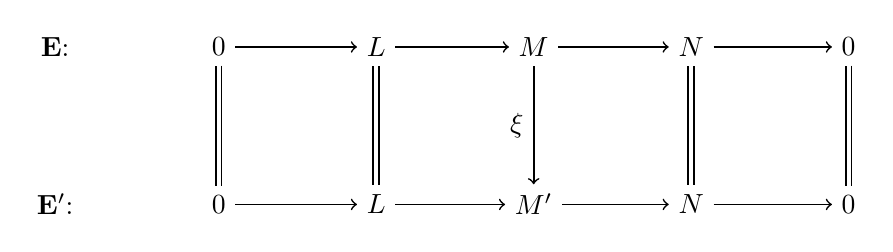
\begin{tikzpicture}[->,-latex, auto, main path/.style={->, semithick}, main node/.style={}]
\node	[main node]		(1) at (0,0)		{$\mathbf{E}$: \quad };
\node	[main node]		(2) at (2,0)		{$0$};
\node	[main node]		(3) at (4,0)		{$L$};
\node [main node]		(4) at (6,0)		{$M$};
\node [main node]		(5) at (8,0)		{$N$};
\node	[main node]		(11) at (10,0)	{$0$};

\node	[main node]		(6) at (0,-2)		{$\mathbf{E'}$: \quad};
\node	[main node]		(7) at (2,-2)		{$0$};
\node	[main node]		(8) at (4,-2)		{$L$};
\node [main node]		(9) at (6,-2)		{$M'$};
\node [main node]		(10) at (8,-2)	{$N$};
\node [main node]		(13) at (10,-2)	{$0$};

\draw (2) edge [main path] node [auto] {$$} (3);
\draw (3) edge [main path] node [auto] {$$} (4);
\draw (4) edge [main path] node [auto] {$$} (5);
\draw (5) edge [main path] (11);

\draw (7) edge [main path] node [auto] {$$} (8);
\draw (8) edge [main path] node [auto] {$$} (9);
\draw (9) edge [main path] node [auto] {$$} (10);
\draw (10) edge [main path] (13);

\draw (3) edge [-, semithick, double, double distance=1.5pt] (8);
\draw (4) edge [main path] node [auto, swap] {$\xi$} (9);
\draw (5) edge [-, semithick, double, double distance=1.5pt](10);
\draw (11) edge [-, semithick, double, double distance=1.5pt] (13);
\draw (2) edge [-, semithick, double, double distance=1.5pt] (7);
\end{tikzpicture}
\end{equation*}
commutes.
\end{mydef}

\begin{eg}
Consider the two short exact sequences, 
\begin{equation*}
\mathbf{E}: \quad 0\xrightarrow{}K\xrightarrow{f}K^2\xrightarrow{g}K\xrightarrow{}0  \quad \& \quad \mathbf{E'}: \quad 0\xrightarrow{}K\xrightarrow{f'}K^2\xrightarrow{g'}K\xrightarrow{}0 ,
\end{equation*}
where $f: x \mapsto (x, 0)$, $g: (x,y)\mapsto y$, $f':x \mapsto (0,x)$ and $g':(x,y)\mapsto x$. Then we can construct the diagram: 
\begin{equation*}
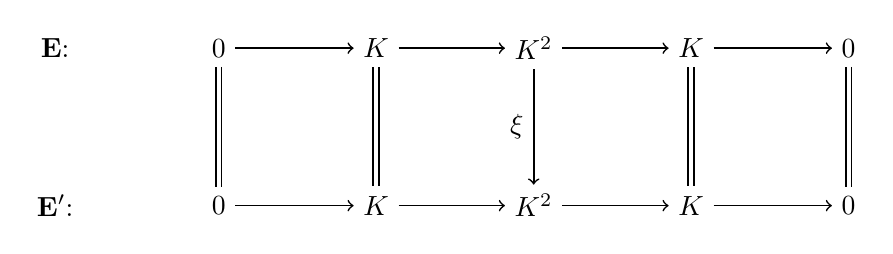
\begin{tikzpicture}[->,-latex, auto, main path/.style={->, semithick}, main node/.style={}]
\node	[main node]		(1) at (0,0)		{$\mathbf{E}$: \quad };
\node	[main node]		(2) at (2,0)		{$0$};
\node	[main node]		(3) at (4,0)		{$K$};
\node [main node]		(4) at (6,0)		{$K^2$};
\node [main node]		(5) at (8,0)		{$K$};
\node	[main node]		(11) at (10,0)	{$0$};

\node	[main node]		(6) at (0,-2)		{$\mathbf{E'}$: \quad};
\node	[main node]		(7) at (2,-2)		{$0$};
\node	[main node]		(8) at (4,-2)		{$K$};
\node [main node]		(9) at (6,-2)		{$K^2$};
\node [main node]		(10) at (8,-2)	{$K$};
\node [main node]		(13) at (10,-2)	{$0$};



\draw (2) edge [main path] node [auto] {$$} (3);
\draw (3) edge [main path] node [auto] {$$} (4);
\draw (4) edge [main path] node [auto] {$$} (5);
\draw (5) edge [main path] (11);


\draw (7) edge [main path] node [auto] {$$} (8);
\draw (8) edge [main path] node [auto] {$$} (9);
\draw (9) edge [main path] node [auto] {$$} (10);
\draw (10) edge [main path] (13);

\draw (3) edge [-, semithick, double, double distance=1.5pt] (8);
\draw (4) edge [main path] node [auto, swap] {$\xi$} (9);
\draw (5) edge [-, semithick, double, double distance=1.5pt](10);
\draw (11) edge [-, semithick, double, double distance=1.5pt] (13);
\draw (2) edge [-, semithick, double, double distance=1.5pt] (7);
\end{tikzpicture}
\end{equation*}
This diagram commutes when $\xi$ is the map $\xi: K^2 \to K^2$, $(x, y) \mapsto (y, x)$, hence these two short exact equations are equivalent.
\end{eg}

For a nonexample we turn to Exercise \uppercase\expandafter{\romannumeral 3} 1.1 in \cite{Stamm}.

\begin{eg}
Consider the two short exact sequences, 
\begin{equation*}
\mathbf{E}: \quad 0\xrightarrow{}\bb{Z}\xrightarrow{f}\bb{Z}\xrightarrow{g}\frac{\bb{Z}}{3\bb{Z}}\xrightarrow{}0  \quad \& \quad \mathbf{E'}: \quad 0\xrightarrow{}\bb{Z}\xrightarrow{f'}\bb{Z}\xrightarrow{g'}\frac{\bb{Z}}{3\bb{Z}}\xrightarrow{}0 ,
\end{equation*}
where $f, f': x\mapsto 3x$, $g: x \mapsto x(\text{mod }3)$ and $g':x\mapsto 2x(\text{mod }3)$. Then we can construct the diagram: 
\begin{equation*}
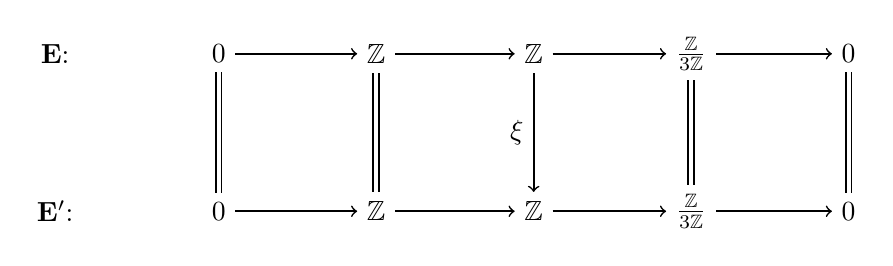
\begin{tikzpicture}[->,-latex, auto, main path/.style={->, semithick}, main node/.style={}]
\node	[main node]		(1) at (0,0)		{$\mathbf{E}$: \quad };
\node	[main node]		(2) at (2,0)		{$0$};
\node	[main node]		(3) at (4,0)		{$\bb{Z}$};
\node [main node]		(4) at (6,0)		{$\bb{Z}$};
\node [main node]		(5) at (8,0)		{$\frac{\bb{Z}}{3\bb{Z}}$};
\node	[main node]		(11) at (10,0)	{$0$};

\node	[main node]		(6) at (0,-2)		{$\mathbf{E'}$: \quad};
\node	[main node]		(7) at (2,-2)		{$0$};
\node	[main node]		(8) at (4,-2)		{$\bb{Z}$};
\node [main node]		(9) at (6,-2)		{$\bb{Z}$};
\node [main node]		(10) at (8,-2)	{$\frac{\bb{Z}}{3\bb{Z}}$};
\node [main node]		(13) at (10,-2)	{$0$};

\draw (2) edge [main path] node [auto] {$$} (3);
\draw (3) edge [main path] node [auto] {$$} (4);
\draw (4) edge [main path] node [auto] {$$} (5);
\draw (5) edge [main path] (11);


\draw (7) edge [main path] node [auto] {$$} (8);
\draw (8) edge [main path] node [auto] {$$} (9);
\draw (9) edge [main path] node [auto] {$$} (10);
\draw (10) edge [main path] (13);

\draw (3) edge [-, semithick, double, double distance=1.5pt] (8);
\draw (4) edge [main path] node [auto, swap] {$\xi$} (9);
\draw (5) edge [-, semithick, double, double distance=1.5pt](10);
\draw (11) edge [-, semithick, double, double distance=1.5pt] (13);
\draw (2) edge [-, semithick, double, double distance=1.5pt] (7);
\end{tikzpicture}
\end{equation*}
Assume $\mathbf{E}$ and $\mathbf{E'}$ are equivalent, so we there must exist some $\xi$ such that the diagram commutes. The second square in the diagram will commute if and only if $\xi=id_{\bb{Z}}$, since $f=f'$, however, this then means the third square will never commute, as $g\neq g'$. Thus no such $\xi$ exists and the two short exact sequences are not equivalent.
\end{eg}

For the discussion of split exact sequences, this report will first follow \cite{Schiff} in defining a section and refraction and then use Schiffler's Proposition 1.8 to prove that the conditions in Definition 1.23 in \cite{CB1} are equivalent. This will obtain us the Splitting Lemma. However, the proof of Proposition 1.8 will be ommitted as it is 

\begin{mydef} \label{secretdef}
\begin{itemize}
\item A map $f: L \to M$ is called a \emph{section} if there exists a map $h: M \to L$ such that $hf=id_L$.
\item A map $g:M\to N$ is called a \emph{retraction} if there exists a map $h: N \to M$ such that $gh=id_N$.
\end{itemize}
\end{mydef}

\begin{mydef}
A short exact sequence,
\begin{equation*}
0\xrightarrow{}L\xrightarrow{f} M \xrightarrow{g} N \xrightarrow{} 0,
\end{equation*}
is said to be \emph{split} if $f$ is a section.
\end{mydef}

\begin{lem} \label{splittinglem} (Splitting Lemma)
If the short exact sequence, 
\begin{equation*}
0\xrightarrow{}L\xrightarrow{f} M \xrightarrow{g} N \xrightarrow{} 0,
\end{equation*}
is split then the following equivalent conditions hold:
\begin{description}
\item [(i)] $f$ is a section.
\item [(ii)] $g$ is a retraction.
\item [(iii)] $im(f)$ is a direct summand of $M$.
\end{description}
\end{lem}
\begin{proof}
Proof omitted. See Proposition 1.8 in \cite{Schiff} and the proof given on \cite{Splittinglem}.
\end{proof}

\begin{eg}
The short exact sequence, 
\begin{equation*}
0 \xrightarrow{}\bb{Z} \xrightarrow{f} \bb{Z}^2 \xrightarrow{g} \bb{Z} \xrightarrow{} 0,
\end{equation*}
where $f: x \mapsto (x, 0)$ and $g: (x, y) \mapsto y$, splits. Then
\begin{description}
\item [(i)] $f$ is a section as the map $h:\bb{Z}^2 \to \bb{Z}$, $(x, y) \mapsto x$ satifies $hf=id_{\bb{Z}}$.
\item [(ii)] $g$ is a retraction as the map $h': \bb{Z} \to \bb{Z}^2$, $y \mapsto (x, y)$ satifies $gh=id_{\bb{Z}}$.
\item [(iii)] $im(f) \cong \bb{Z}$ is a direct summand of $\bb{Z}^2 \cong \bb{Z}\oplus \bb{Z}$.
\end{description}
\end{eg}

Rather than provide the following result as a proposition and prove it directly as Rotman does in \cite{Rotman}, it will be given as a corollary of the splitting lemma as in \cite{Schiff}.

\begin{cor} \label{MLNcor}
If the sequence,
\begin{equation*}
0\xrightarrow{}L\xrightarrow{f} M \xrightarrow{g} N \xrightarrow{} 0,
\end{equation*}
is split exact, then
\begin{equation*}
M \cong L \oplus N.
\end{equation*}
\end{cor}
\begin{proof}
Since $f$ is injective as the seqence is short exact, we have $L \cong im(f) \cong ker(g)$. The since $g$ is surjective as the sequence is short exact, the first isomorphism theorem implies $N \cong \sfrac{M}{ker(g)}$. Then Lemma \ref{splittinglem} gives $M$  is a direct summand of $im(f)$, hence, $M\cong L \oplus N$.
\end{proof}

\begin{eg}
Notice that in the previous example $\bb{Z} \cong im(f)\cong ker(g) $ and $\bb{Z} \cong \sfrac{\bb{Z}^2}{ker(g)}\cong \bb{Z}$. Hence, $\bb{Z}^2 \cong \bb{Z} \oplus \bb{Z}$, as expected.
\end{eg}


\begin{mydef} \label{pushoutdef}
Given a short exact seqence,
\begin{equation*}
\mathbf{E}: \qquad 0\xrightarrow{}L\xrightarrow{f} M \xrightarrow{g} N \xrightarrow{} 0,
\end{equation*}
and a map $\theta : L \to L'$ then the short exact sequence, 
\begin{equation*}
\mathbf{E'}: \qquad 0\xrightarrow{} L' \xrightarrow{f'} M' \xrightarrow{g'} N \xrightarrow{}0,
\end{equation*}
fitting into the commutative diagram
\begin{equation*}
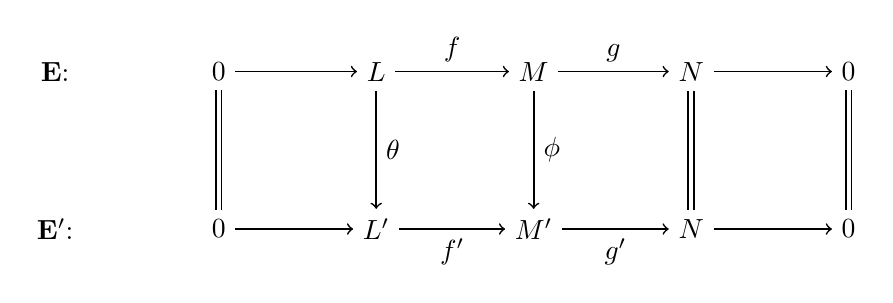
\begin{tikzpicture}[->,-latex, auto, main path/.style={->, semithick}, main node/.style={}]
\node	[main node]		(1) at (0,0)		{$\mathbf{E}$: \quad };
\node	[main node]		(2) at (2,0)		{$0$};
\node	[main node]		(3) at (4,0)		{$L$};
\node [main node]		(4) at (6,0)		{$M$};
\node [main node]		(5) at (8,0)		{$N$};
\node	[main node]		(11) at (10,0)	{$0$};

\node	[main node]		(6) at (0,-2)		{$\mathbf{E'}$: \quad};
\node	[main node]		(7) at (2,-2)		{$0$};
\node	[main node]		(8) at (4,-2)		{$L'$};
\node [main node]		(9) at (6,-2)		{$M'$};
\node [main node]		(10) at (8,-2)	{$N$};
\node [main node]		(13) at (10,-2)	{$0$};

\draw (2) edge [main path] node [auto] {$$} (3);
\draw (3) edge [main path] node [auto] {$f$} (4);
\draw (4) edge [main path] node [auto] {$g$} (5);
\draw (5) edge [main path] (11);

\draw (7) edge [main path] node [auto] {$$} (8);
\draw (8) edge [main path] node [auto, swap] {$f'$} (9);
\draw (9) edge [main path] node [auto, swap] {$g'$} (10);
\draw (10) edge [main path] (13);

\draw (3) edge [main path] node [auto] {$\theta$} (8);
\draw (4) edge [main path] node [auto] {$\phi$} (9);
\draw (5) edge [-, semithick, double, double distance=1.5pt](10);
\draw (11) edge [-, semithick, double, double distance=1.5pt] (13);
\draw (2) edge [-, semithick, double, double distance=1.5pt] (7);
\end{tikzpicture}
\end{equation*}
is defined to be the \emph{pushout of $\mathbf{E}$ along $\theta$}.
\end{mydef}

\begin{prop} \label{pushoutprop}
Let $\mathbf{E}$, $\mathbf{E'}$ and $\theta: L \to L'$ be defined as above in Definition \ref{pushoutdef}. Then the pushout of $\mathbf{E}$ along $\theta$ exists and is unique up to equivalence.
\end{prop}
\begin{proof}
Existence: Firstly, set
\begin{equation*}
M'=\frac{(L'\oplus M)}{\{(\theta(l), -f(l)): l\in L\}},
\end{equation*}
and let the maps be $f': l'\mapsto \overline{(l',0)}$, $g': \overline{(l',m)}\mapsto g(m)$ and $\phi: m \mapsto \overline{(0,m)}$, where $\overline{(l',m)}$ denotes the class of $(l', m) \in L'\oplus M$ in $M'$. The diagram is then commutative as $\phi(f(l))=\overline{(0,f(l))}=\overline{(0,0)}=\overline{(\theta(l),0)}=f'(\theta(l))$ for an $l\in L$ and $id_N(g(m))=g(m)=g'(\theta(m))$ for any $m\in M$. The pushout is exact as $im(f')=\{\overline{(l',0)}:l'\in L'\}=ker(g')$.\\
Uniqueness: The sequence
\begin{equation*}
\mathbf{\xi'} \qquad 0\xrightarrow{}L \xrightarrow{\begin{psmallmatrix}\theta \\ -f \end{psmallmatrix}} L'\oplus M \xrightarrow{\begin{psmallmatrix} f' & \phi \end{psmallmatrix}} M' \xrightarrow{} 0,
\end{equation*}
is exact as $im(\begin{psmallmatrix}\theta \\ -f \end{psmallmatrix})=\{\begin{psmallmatrix}\theta(l) \\ -f(l) \end{psmallmatrix}: l \in L\}=ker(\begin{psmallmatrix} f' & \phi \end{psmallmatrix})$. Exactness then implies that $\begin{psmallmatrix} f' & \phi \end{psmallmatrix}$ is surjective and so by the first isomorphism theorem (see proof of Corollary \ref{MLNcor}) we have,
\begin{equation*}
M' \cong \frac{L'\oplus M}{ker(\begin{psmallmatrix} f' & \phi \end{psmallmatrix})} \cong \frac{L'\oplus M}{\{(\theta(l), -f(l)): l\in L\}}.
\end{equation*}
This gives equivalence between $\mathbf{E'}$ and $\mathbf{E''}$.
\end{proof}

\begin{eg}
Consider the short exact sequence,
\begin{equation*}
\mathbf{E}: \qquad 0\xrightarrow{} \bb{Z} \xrightarrow[f]{n} \bb{Z}\xrightarrow[g]{nat}\frac{\bb{Z}}{n\bb{Z}} \xrightarrow{} 0,
\end{equation*}
and the $\bb{Z}$-module map $\theta: \bb{Z} \to \sfrac{\bb{Z}}{n\bb{Z}}$ is the natural one. Now we can use Proposition \ref{pushoutprop} to construct the pushout of $\mathbf{E}$ along $\theta$.\\
Firstly, construct the commutative diagram,
\begin{equation*}
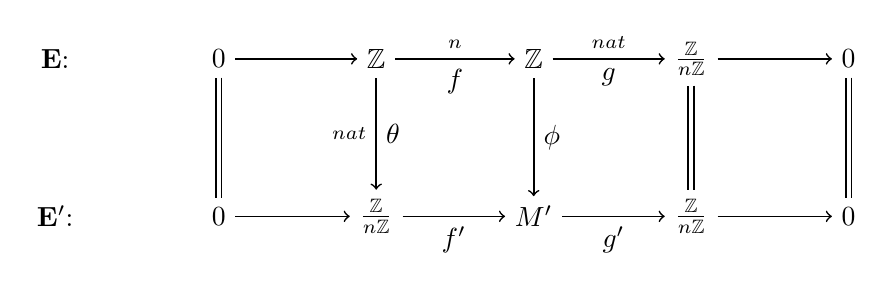
\begin{tikzpicture}[->,-latex, auto, main path/.style={->, semithick}, main node/.style={}]
\node	[main node]		(1) at (0,0)		{$\mathbf{E}$: \quad };
\node	[main node]		(2) at (2,0)		{$0$};
\node	[main node]		(3) at (4,0)		{$\bb{Z}$};
\node [main node]		(4) at (6,0)		{$\bb{Z}$};
\node [main node]		(5) at (8,0)		{$\frac{\bb{Z}}{n\bb{Z}}$};
\node	[main node]		(11) at (10,0)	{$0$};

\node	[main node]		(6) at (0,-2)		{$\mathbf{E'}$: \quad};
\node	[main node]		(7) at (2,-2)		{$0$};
\node	[main node]		(8) at (4,-2)		{$\frac{\bb{Z}}{n\bb{Z}}$};
\node [main node]		(9) at (6,-2)		{$M'$};
\node [main node]		(10) at (8,-2)	{$\frac{\bb{Z}}{n\bb{Z}}$};
\node [main node]		(13) at (10,-2)	{$0$};

\draw (2) edge [main path] node [auto] {$$} (3);
\draw (3) edge [main path] node [auto] {$\scriptstyle{n}$} node [auto, swap] {$f$} (4);
\draw (4) edge [main path] node [auto] {$\scriptstyle{nat}$} node [auto, swap] {$g$} (5);
\draw (5) edge [main path] (11);

\draw (7) edge [main path] node [auto] {$$} (8);
\draw (8) edge [main path] node [auto, swap] {$f'$} (9);
\draw (9) edge [main path] node [auto, swap] {$g'$} (10);
\draw (10) edge [main path] (13);

\draw (3) edge [main path] node [auto] {$\theta$} node [auto, swap] {$\scriptstyle{nat}$} (8);
\draw (4) edge [main path] node [auto] {$\phi$} (9);
\draw (5) edge [-, semithick, double, double distance=1.5pt](10);
\draw (11) edge [-, semithick, double, double distance=1.5pt] (13);
\draw (2) edge [-, semithick, double, double distance=1.5pt] (7);
\end{tikzpicture}
\end{equation*}
and now we want to find $M'$. As $\theta: x \mapsto x+n\bb{Z}$ and $f: x \mapsto nx$, we have,
\begin{equation*}
M'=\frac{\frac{\bb{Z}}{n\bb{Z}}\oplus\bb{Z}}{\{(x+n\bb{Z}, -nx):x \in \bb{Z}\}},
\end{equation*}
and we can set $f': \sfrac{\bb{Z}}{n\bb{Z}} \to M'$, $x+n\bb{Z} \mapsto \overline{(x+n\bb{Z},0)}$, $g': M' \to \sfrac{\bb{Z}}{n\bb{Z}}$, $\overline{(x+n\bb{Z}, y)} \mapsto y+n\bb{Z}$, and $\phi: \bb{Z} \to M'$, $x \mapsto \overline{(0,x)}$. It is clear that this makes the above diagram commutative and gives $\mathbf{E'}$ exact. Furthermore, the map $\phi$ is onto as,
\begin{align*}
M'\ni\overline{(x+n\bb{Z}, y)}&=\overline{(x+n\bb{Z}, -nx)} + \overline{(o, y+na)},\\
&=\overline{(0, y+nx)} \in im(\phi).
\end{align*}
We can also see that, 
\begin{align*}
ker(\phi)&= \{y\in \bb{Z}: \overline{(0, y)}=0\},\\
&=\{y\in \bb{Z}: \overline{(0, y)} \text{ is of the form } \overline{(x+n\bb{Z}, -nx)}\},\\
&=\{y\in \bb{Z}: n|y\text{, }x=\frac{-b}{n}\text{ and } x+n\bb{Z}=0\},\\
&=\{y\in \bb{Z}: n^2|y\}\cong n^2\bb{Z},
\end{align*}
and then the First Isomorphism Theorem gives, 
\begin{equation*}
M'\cong \frac{\bb{Z}}{ker(\phi)}\cong \frac{\bb{Z}}{n^2\bb{Z}}.
\end{equation*}
Hence, the pushout of $\mathbf{E}$ along $\theta$ is,
\begin{equation*}
\mathbf{E'}: \qquad 0\xrightarrow{} \frac{\bb{Z}}{n\bb{Z}} \xrightarrow{f'} \frac{\bb{Z}}{n^2\bb{Z}}\xrightarrow{g'} \frac{\bb{Z}}{n\bb{Z}} \xrightarrow{} 0,
\end{equation*}
with the maps $f', g'$ defined as above.
\end{eg}

\begin{mydef} \label{pullbackdef}
Given a short exact seqence,
\begin{equation*}
\mathbf{E}: \qquad 0\xrightarrow{}L\xrightarrow{f} M \xrightarrow{g} N \xrightarrow{} 0,
\end{equation*}
and a map $\psi: N''\to N$ then the short exact sequence, 
\begin{equation*}
\mathbf{E''}: \qquad 0\xrightarrow{} L \xrightarrow{f''} M'' \xrightarrow{g''} N'' \xrightarrow{}0,
\end{equation*}
fitting into the commutative diagram
\begin{equation*}
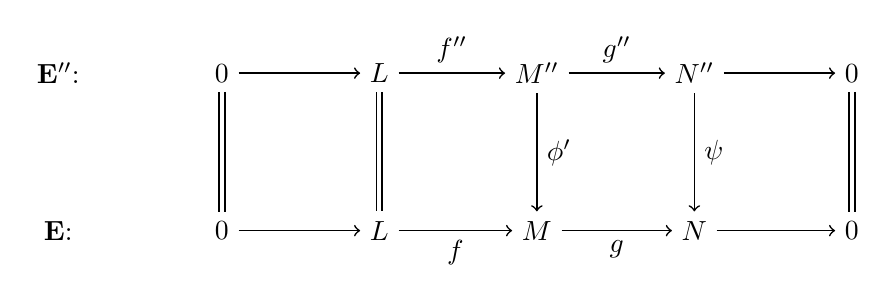
\begin{tikzpicture}[->,-latex, auto, main path/.style={->, semithick}, main node/.style={}]
\node	[main node]		(1) at (0,0)		{$\mathbf{E''}$: \quad };
\node	[main node]		(2) at (2,0)		{$0$};
\node	[main node]		(3) at (4,0)		{$L$};
\node [main node]		(4) at (6,0)		{$M''$};
\node [main node]		(5) at (8,0)		{$N''$};
\node	[main node]		(11) at (10,0)	{$0$};

\node	[main node]		(6) at (0,-2)		{$\mathbf{E}$: \quad};
\node	[main node]		(7) at (2,-2)		{$0$};
\node	[main node]		(8) at (4,-2)		{$L$};
\node [main node]		(9) at (6,-2)		{$M$};
\node [main node]		(10) at (8,-2)	{$N$};
\node [main node]		(13) at (10,-2)	{$0$};

\draw (2) edge [main path] node [auto] {$$} (3);
\draw (3) edge [main path] node [auto] {$f''$} (4);
\draw (4) edge [main path] node [auto] {$g''$} (5);
\draw (5) edge [main path] (11);

\draw (7) edge [main path] node [auto] {$$} (8);
\draw (8) edge [main path] node [auto, swap] {$f$} (9);
\draw (9) edge [main path] node [auto, swap] {$g$} (10);
\draw (10) edge [main path] (13);

\draw (3) edge [-, semithick, double, double distance=1.5pt] (8);
\draw (4) edge [main path] node [auto] {$\phi'$} (9);
\draw (5) edge[main path] node [auto] {$\psi$} (10);
\draw (11) edge [-, semithick, double, double distance=1.5pt] (13);
\draw (2) edge [-, semithick, double, double distance=1.5pt] (7);
\end{tikzpicture}
\end{equation*}
is defined to be the \emph{pullback} of $\mathbf{E}$ along $\psi$.
\end{mydef}

\begin{prop} \label{pullbackprop}
Let $\mathbf{E}$, $\mathbf{E''}$ and $\psi: N''\to N$ be defined as above in Definition \ref{pullbackdef}. Then the pullback of $\mathbf{E}$ along $\psi$ exists and is unique up to equivalence.
\end{prop}
\begin{proof}
Existence: Firstly, set
\begin{equation*}
M''=\{(m,n'')\in M\oplus N'': g(m)=\psi(n'')\},
\end{equation*}
and let the maps be $f'': L \to M''$, $l\mapsto (f(l),0)$ (if $g(f(l))=\psi(0)$, $0$ otherwise), $g'': M'' \to N''$, $(m, n'') \mapsto n''$, and $\phi': M'' \to M$, $(m, n'') \mapsto m$. The diagram is then commutative by diagram chasing and the pullback is exact as $im(f)=\{(f(l),0):l\in L\text{ and } g(f(l))=\psi(0)\}=\{(m, 0): m \in M\text{ and }g(m)=\psi(0)\}=ker(g'')$. 
Uniqueness: Consider the commutative diagram of short exact sequences,
\begin{equation*}
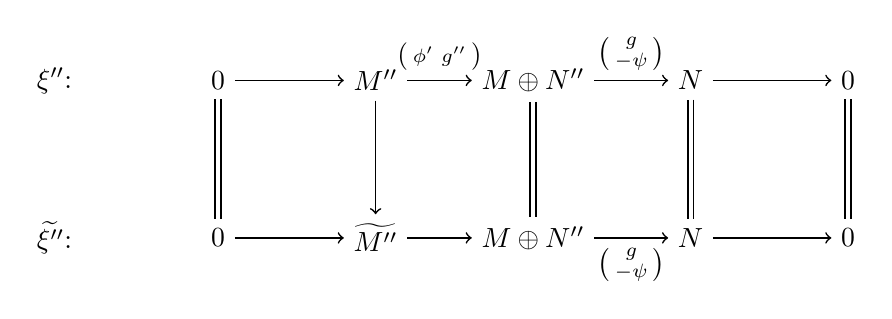
\begin{tikzpicture}[->,-latex, auto, main path/.style={->, semithick}, main node/.style={}]
\node	[main node]		(1) at (0,0)		{$\mathbf{\xi''}$: \quad };
\node	[main node]		(2) at (2,0)		{$0$};
\node	[main node]		(3) at (4,0)		{$M''$};
\node [main node]		(4) at (6,0)		{$M\oplus N''$};
\node [main node]		(5) at (8,0)		{$N$};
\node	[main node]		(11) at (10,0)	{$0$};

\node	[main node]		(6) at (0,-2)		{$\mathbf{\widetilde{\xi''}}$: \quad};
\node	[main node]		(7) at (2,-2)		{$0$};
\node	[main node]		(8) at (4,-2)		{$\widetilde{M''}$};
\node [main node]		(9) at (6,-2)		{$M\oplus N''$};
\node [main node]		(10) at (8,-2)	{$N$};
\node [main node]		(13) at (10,-2)	{$0$};

\draw (2) edge [main path] node [auto] {$$} (3);
\draw (3) edge [main path] node [auto] {$\begin{psmallmatrix}\phi' & g''\end{psmallmatrix}$} (4);
\draw (4) edge [main path] node [auto] {$\begin{psmallmatrix}g \\ -\psi \end{psmallmatrix}$} (5);
\draw (5) edge [main path] (11);

\draw (7) edge [main path] node [auto] {$$} (8);
\draw (8) edge [main path] node [auto, swap] {$$} (9);
\draw (9) edge [main path] node [auto, swap] {$\begin{psmallmatrix}g \\ -\psi \end{psmallmatrix}$} (10);
\draw (10) edge [main path] (13);

\draw (3) edge [main path] node [auto] {$$} (8);
\draw (4) edge [-, semithick, double, double distance=1.5pt] (9);
\draw (5) edge [-, semithick, double, double distance=1.5pt](10);
\draw (11) edge [-, semithick, double, double distance=1.5pt] (13);
\draw (2) edge [-, semithick, double, double distance=1.5pt] (7);
\end{tikzpicture}
\end{equation*}
where $M''$ and $\widetilde{M''}$ are from two pullbacks, $\mathbf{E''}$ and $\mathbf{\widetilde{E''}}$, of $\mathbf{E}$ along $\psi$. By diagram chasing we can see that there is in fact an isomorphism between $M''$ and $\widetilde{M''}$ and so $\mathbf{E''}$ and $\mathbf{\widetilde{E''}}$ are equivalent as short exact sequences.
\end{proof}

\begin{eg}
Consider the short exact sequence, 
\begin{equation*}
\mathbf{E}: \qquad 0\xrightarrow{} \bb{Z} \xrightarrow[f]{n} \bb{Z}\xrightarrow[g]{nat}\frac{\bb{Z}}{n\bb{Z}} \xrightarrow{} 0,
\end{equation*}
and the $\bb{Z}$-module map $\psi: \bb{Z} \to \sfrac{\bb{Z}}{n\bb{Z}}$ is the natural one. Now we can use Proposition \ref{pullbackprop} to construct the pullback of $\mathbf{E}$ along $\psi$.\\
Firstly, construct the commutative diagram,
\begin{equation*}
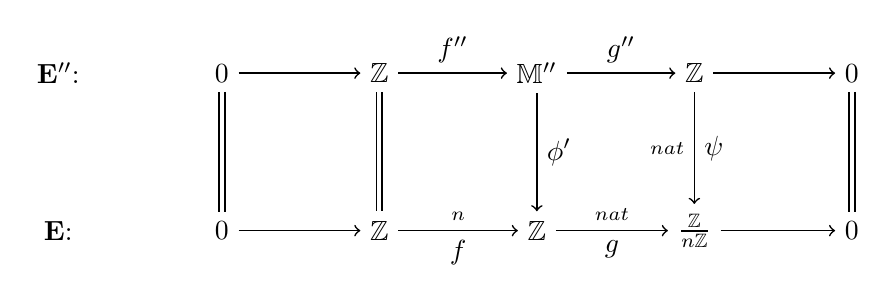
\begin{tikzpicture}[->,-latex, auto, main path/.style={->, semithick}, main node/.style={}]
\node	[main node]		(1) at (0,0)		{$\mathbf{E''}$: \quad };
\node	[main node]		(2) at (2,0)		{$0$};
\node	[main node]		(3) at (4,0)		{$\bb{Z}$};
\node [main node]		(4) at (6,0)		{$\bb{M''}$};
\node [main node]		(5) at (8,0)		{$\bb{Z}$};
\node	[main node]		(11) at (10,0)	{$0$};

\node	[main node]		(6) at (0,-2)		{$\mathbf{E}$: \quad};
\node	[main node]		(7) at (2,-2)		{$0$};
\node	[main node]		(8) at (4,-2)		{$\bb{Z}$};
\node [main node]		(9) at (6,-2)		{$\bb{Z}$};
\node [main node]		(10) at (8,-2)	{$\frac{\bb{Z}}{n\bb{Z}}$};
\node [main node]		(13) at (10,-2)	{$0$};

\draw (2) edge [main path] node [auto] {$$} (3);
\draw (3) edge [main path]node [auto] {$f''$} (4);
\draw (4) edge [main path] node [auto] {$g''$} (5);
\draw (5) edge [main path] (11);

\draw (7) edge [main path] node [auto] {$$} (8);
\draw (8) edge [main path]  node [auto] {$\scriptstyle{n}$} node [auto, swap] {$f$} (9);
\draw (9) edge [main path] node [auto] {$\scriptstyle{nat}$}  node [auto, swap] {$g$} (10);
\draw (10) edge [main path] (13);

\draw (3) edge  [-, semithick, double, double distance=1.5pt](8);
\draw (4) edge [main path] node [auto] {$\phi'$} (9);
\draw (5) edge [main path] node [auto] {$\psi$} node [auto, swap] {$\scriptstyle{nat}$} (10);
\draw (11) edge [-, semithick, double, double distance=1.5pt] (13);
\draw (2) edge [-, semithick, double, double distance=1.5pt] (7);
\end{tikzpicture}
\end{equation*}
and now to find $M''$. As both $\psi, g: x \mapsto x+n\bb{Z}$, we have,
\begin{align*}
M''&=\{(x,y) \in \bb{Z} \oplus \bb{Z} : x+n\bb{Z}=y+n\bb{Z}\}, \\
&=\{(x, y) \in \bb{Z} \oplus \bb{Z}: n\divides x-y\}, \\
&= \frac{\bb{Z}\oplus\bb{Z}}{\{(x, y): n\ndivides x-y\}},
\end{align*}
and we can set $f'': \bb{Z} \to M''$, $x \mapsto \overline{(nx, 0)}$, $g'': M'' \to \bb{Z}$, $\overline{(x, y)} \mapsto y$ and $\phi': M'' \to \bb{Z}$, $\overline(x, y) \mapsto m$. It is clear that this makes the diagram commutative and gives $\mathbf{E''}$ exact. 
% Need to find a way of working out what M'' is isomorphic to
\end{eg}

Now this report will start to consider the results possible by considering exact sequences of ....\\
%FILL THIS IN 
% Put in Weibel Exercise 1.3.1
% Add fives lemma??
The following theorem is from \cite{CB1}, however, the notation has been changed to make the different maps more explicit and more detail is given in the proof. 

\begin{thm} (Long Exact Sequence) \label{longexactseqthm} \\
Let $0\xrightarrow{}\mathbf{C} \xrightarrow{f} \mathbf{D} \xrightarrow{g} \mathbf{E} \xrightarrow{}0$ be a short exact sequence of chain complexes, meaning that $f$ and $g$ are chain maps and for each $n$ the maps
\begin{equation*}
0 \xrightarrow{} C_n \xrightarrow{f_n} D_n \xrightarrow{g_n} E_n \xrightarrow{} 0,
\end{equation*}
form a short exact sequence. Then there are connecting maps $c_n:H_n(\mathbf{E}) \to H_{n-1}(\mathbf{C})$ giving a long exact sequence, 
\begin{equation*}
\dots \xrightarrow{}H_{n+1}(\mathbf{E}) \xrightarrow{c_{n+1}} H_n(\mathbf{C}) \xrightarrow{} H_n(\mathbf{D})\xrightarrow{}H_n(\mathbf{E}) \xrightarrow{c_n} H_{n-1}(\mathbf{C}) \xrightarrow{} H_{n-1}(\mathbf{D}) \xrightarrow{} \dots
\end{equation*}
\end{thm}
\begin{proof}
Have diagram,
\begin{equation*}
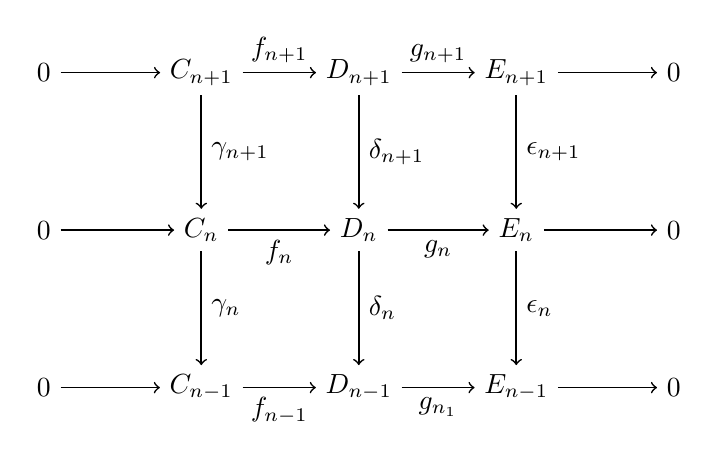
\begin{tikzpicture}[->,-latex, auto, main path/.style={->, semithick}, main node/.style={}]

\node	[main node]		(2) at (2,0)		{$0$};
\node	[main node]		(3) at (4,0)		{$C_{n+1}$};
\node [main node]		(4) at (6,0)		{$D_{n+1}$};
\node [main node]		(5) at (8,0)		{$E_{n+1}$};
\node	[main node]		(11) at (10,0)	{$0$};


\node	[main node]		(7) at (2,-2)		{$0$};
\node	[main node]		(8) at (4,-2)		{$C_n$};
\node [main node]		(9) at (6,-2)		{$D_n$};
\node [main node]		(10) at (8,-2)	{$E_n$};
\node [main node]		(13) at (10,-2)	{$0$};


\node	[main node]		(14) at (2,-4)	{$0$};
\node	[main node]		(15) at (4,-4)	{$C_{n-1}$};
\node [main node]		(16) at (6,-4)	{$D_{n-1}$};
\node [main node]		(17) at (8,-4)	{$E_{n-1}$};
\node [main node]		(18) at (10,-4)	{$0$};

\draw (2) edge [main path] node [auto] {$$} (3);
\draw (3) edge [main path] node [auto] {$f_{n+1}$} (4);
\draw (4) edge [main path] node [auto] {$g_{n+1}$} (5);
\draw (5) edge [main path] (11);

\draw (7) edge [main path] node [auto] {$$} (8);
\draw (8) edge [main path] node [auto, swap] {$f_n$} (9);
\draw (9) edge [main path] node [auto, swap] {$g_n$} (10);
\draw (10) edge [main path] (13);

\draw (14) edge [main path] node [auto] {$$} (15);
\draw (15) edge [main path] node [auto, swap] {$f_{n-1}$} (16);
\draw (16) edge [main path] node [auto, swap] {$g_{n_1}$} (17);
\draw (17) edge [main path] (18);

\draw (3) edge [main path] node [auto] {$\gamma_{n+1}$} (8);
\draw (4) edge [main path] node [auto] {$\delta_{n+1}$} (9);
\draw (5) edge [main path] node [auto] {$\epsilon_{n+1}$} (10);

\draw (8) edge [main path] node [auto] {$\gamma_{n}$} (15);
\draw (9) edge [main path] node [auto] {$\delta_{n}$} (16);
\draw (10) edge [main path] node [auto] {$\epsilon_{n}$} (17);
\end{tikzpicture}
\end{equation*}
Define the connecting map $c_n:H_n(\mathbf{E})\to H_{n-1}(\mathbf{C})$ as follows:\\
Let $\overline{x}$ be a typical element of $H_n(\mathbf{E})$, with $x \in ker(\epsilon_n)=Z_n(\mathbf{E})$. Then as $g_n$ is surjective we can lift $x\in E_n$ to some element $y \in D_n$ such that $g_n(y)=x$. From the commutativity of the diagram, 
\begin{equation*}
g_{n-1}(\delta_n(y))=\epsilon_n(g_n(y))=\epsilon_n(x)=0,
\end{equation*}
since $x\in ker(\epsilon_n)$. Hence, $\delta_n(y)\in ker(g_{n-1})\cong im(f_{n-1})$. Then as $f_{n-1}$ is injective there exists some $z\in C_{n-1}$ such that $f_{n-1}(z)=\delta_n(y)$. Thus define $c_n(\overline{x})=\overline{z}$.(Note $z \in ker(\gamma_{n-1})$ as $\delta_{n-1}(\delta_n(y))=0$, then by commutivity $f_{n-2}(\gamma_{n-1}(z))=0$ and as $f_{n-2}$ is injective.)\\
Now to show not dependent on choice of $x$ or $y$:
Say $y, y'\in D_n$ have images $g_n(y)=x$, $g_n(y')=x'$ where $x, x'\in ker(\epsilon_n)=Z_n(\mathbf{E})$ with $\overline{x}=\overline{x'}$. Thus $g_n(y)-g_n(y')\in im(\epsilon_{n+1})=B_n(\mathbf{E})$. Therefore, 
\begin{align*}
g_n(y-y')&=\epsilon_{n+1}(g_{n+1}(u))\text{, for some }u\in D_{n+1},\\
&=g_n(\delta_{n+1}(u)).
\end{align*}
Hence, $y-y'-\delta_{n+1}(u)=f_n(v)$ for some $v\in C_n$ by the injectivity of $f_n$. \\
If $f_{n-1}(z)=\delta_n(y)$ and $f_{n-1}(z')=\delta_n(y')$ then,
\begin{align*}
f_{n-1}(z-z')&=\delta_n(y-y'),\\
&=\delta_n(y-y'-\delta_(u))\text{, as $\delta_n(\delta_{n+1}(u))=0$ as chain complex,}\\
&=\delta_n(f_n(v)),\\
&=f_{n-1}(\gamma_n(v)),
\end{align*}
implying $z-z'=\gamma_n(v)\in im(\gamma_n)=B_{n-1}(\mathbf{C})$. Hence, $\overline{z}=\overline{z'}$ in $H_{n-1}(\mathbf{C})$.
%Find out why need to include the bit about it being exact at H_n(D)???
\end{proof}
% Maybe include an example, going to take some time to work one out...

Note that this report is following Crawley-Boevey's example in \cite{CB1} by proving the Long Exact Sequence theorem directly and taking the Snake Lemma as a corollary, unlike in other reading material, like \cite{Weibel} where the Long Exact Sequence is given as a corollary of the Snake Lemma. If the reader would like a direct proof of the Snake Lemma, we direct them, as Weibel does in \cite{Weibel}, to \emph{It's My Turn} (Rastar-Martin Elfand Studios, 1980), where a proof is given in the beginning of the movie.
% This might need a rewrite

\begin{cor} (Snake Lemma)\\
If you have a commutative diagram with exact rows, 
\begin{equation*}
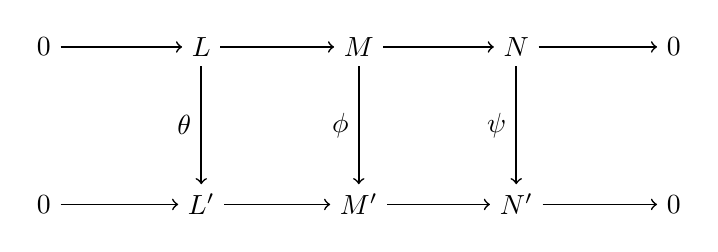
\begin{tikzpicture}[->,-latex, auto, main path/.style={->, semithick}, main node/.style={}]

\node	[main node]		(2) at (2,0)		{$0$};
\node	[main node]		(3) at (4,0)		{$L$};
\node [main node]		(4) at (6,0)		{$M$};
\node [main node]		(5) at (8,0)		{$N$};
\node	[main node]		(11) at (10,0)	{$0$};


\node	[main node]		(7) at (2,-2)		{$0$};
\node	[main node]		(8) at (4,-2)		{$L'$};
\node [main node]		(9) at (6,-2)		{$M'$};
\node [main node]		(10) at (8,-2)	{$N'$};
\node [main node]		(13) at (10,-2)	{$0$};

\draw (2) edge [main path] node [auto] {$$} (3);
\draw (3) edge [main path]node [auto] {$$} (4);
\draw (4) edge [main path] node [auto] {$$} (5);
\draw (5) edge [main path] (11);

\draw (7) edge [main path] node [auto] {$$} (8);
\draw (8) edge [main path] (9);
\draw (9) edge [main path] (10);
\draw (10) edge [main path] (13);


\draw (3) edge [main path] node [auto, swap] {$\theta$} (8);
\draw (4) edge [main path] node [auto, swap] {$\phi$} (9);
\draw (5) edge [main path] node [auto, swap] {$\psi$} (10);

\end{tikzpicture}
\end{equation*}
you get an exact sequence, 
\begin{equation*}
0\xrightarrow{}ker(\theta)\xrightarrow{}ker(\phi)\xrightarrow{}ker(\psi)\xrightarrow{}coker(\theta)\xrightarrow{}coker(\phi)\xrightarrow{}coker(\psi)\xrightarrow{}0
\end{equation*}
\end{cor}
\begin{proof}
Consider $L\to L'$, $M\to M'$ and $N\to N'$ as chain complexes and use Theorem \ref{longexactseqthm}.
\end{proof}

\begin{rem}
A short exact sequence of cochain complexes $0\xrightarrow{}\mathbf{C}\xrightarrow{}\mathbf{D} \xrightarrow{} \mathbf{E}\xrightarrow{}0$ gives a long exact sequence,
\begin{equation*}
\dots \xrightarrow{} H^{n-1}(\mathbf{E})\xrightarrow{}H^n(\mathbf{C})\xrightarrow{}H^n(\mathbf{D})\xrightarrow{}H^n(\mathbf{E})\xrightarrow{} H^{n+1}(\mathbf{C})\xrightarrow{} H^{n+1}(\mathbf{D})\xrightarrow{} \dots
\end{equation*}
by renumbering in Theorem \ref{longexactseqthm}.
\end{rem}

%%%%%%%%%%%%%%%%%%%%%%%%%%%%%%%%%%%%%%%%%%%%%%%%%%%%%%%
%%%%%%%%%%%%%%		 Homotopy and Quasi-Isomorphism 		%%%%%%%%%%%%%%%%%
%%%%%%%%%%%%%%%%%%%%%%%%%%%%%%%%%%%%%%%%%%%%%%%%%%%%%%%

\section{Homotopy and Quasi-Isomorphism}

\begin{mydef}
If $f,g:\mathbf{C} \to \mathbf{D}$  are chain maps, then $f$ and $g$ are \emph{homotopic}, denoted $f\simeq g$, if for each $n$ there are maps $h_n: C_n \to D_{n+1}$ such that,
\begin{equation*}
f_n-g_n=h_{n+1}\gamma_n + \delta_{n+1}h_n,
\end{equation*}
where,
\begin{equation*}
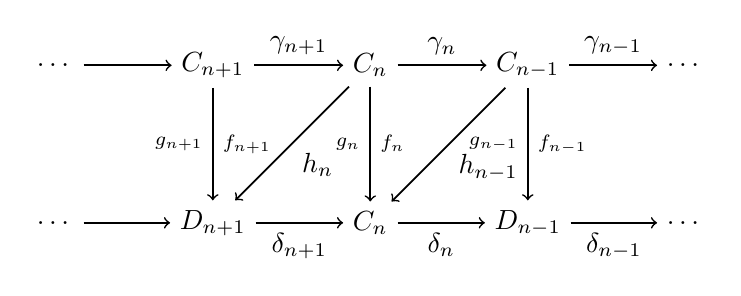
\begin{tikzpicture}[->,-latex, auto, main path/.style={->, semithick}, main node/.style={}]
\node	[main node]		(2) at (2,0)		{\dots};
\node	[main node]		(3) at (4,0)		{$C_{n+1}$};
\node [main node]		(4) at (6,0)		{$C_n$};
\node [main node]		(5) at (8,0)		{$C_{n-1}$};
\node	[main node]		(11) at (10,0)	{\dots};

\node	[main node]		(7) at (2,-2)		{\dots};
\node	[main node]		(8) at (4,-2)		{$D_{n+1}$};
\node [main node]		(9) at (6,-2)		{$C_n$};
\node [main node]		(10) at (8,-2)	{$D_{n-1}$};
\node [main node]		(13) at (10,-2)	{\dots};

\draw (2) edge [main path] node [auto] {$$} (3);
\draw (3) edge [main path] node [auto] {$\gamma_{n+1}$} (4);
\draw (4) edge [main path] node [auto] {$\gamma_n$} (5);
\draw (5) edge [main path] node [auto] {$\gamma_{n-1}$} (11);

\draw (7) edge [main path] node [auto] {$$} (8);
\path (8) edge [main path] node [auto, swap] {$\delta_{n+1}$} (9);
\draw (9) edge [main path] node [auto, swap] {$\delta_n$} (10);
\draw (10) edge [main path] node [auto, swap] {$\delta_{n-1}$} (13);

\draw (3) edge [main path] node [auto] {$\scriptstyle{f_{n+1}}$} node [auto, swap] {$\scriptstyle{g_{n+1}}$} (8);
\draw (4) edge [main path] node [auto] {$\scriptstyle{f_n}$} node [auto, swap] {$\scriptstyle{g_n}$} (9);
\draw (5) edge [main path] node [auto] {$\scriptstyle{f_{n-1}}$} node [auto, swap] {$\scriptstyle{g_{n-1}}$} (10);

\draw (4) edge [main path] node [auto] {$h_n$} (8);
\draw (5) edge [main path] node [auto] {$h_{n-1}$} (9);
\end{tikzpicture}
\end{equation*}
\end{mydef}



%%%%%%%%%%%%%%%%%%%%%%%%%%%%%%%%%%%%%%%%%%%%%%%%%%%%%%%
%%%%%%%%%%%%%%		 Projective and Injective Resolutions 		%%%%%%%%%%%%%%%%%%
%%%%%%%%%%%%%%%%%%%%%%%%%%%%%%%%%%%%%%%%%%%%%%%%%%%%%%%

\section{Projective and Injective Resolutions}

In this section we look at projective and injective modules and resolutions, for this the reader will need some prior knowledge of free modules, which will not be covered in this report. The reader is advised to look at \cite{Stamm}, \cite{Weibel} and \cite{Rotman} for more information regarding free modules.\\
The following properties for projective modules come from \cite{CB1} with added details from either my own work or \cite{Rotman}. In order to have a clear definition of a projective modules, rather than as a culmination of properties, we have promoted the first property from \cite{CB1} to a definition and to aid this we give a separate defintion for a lifting as in \cite{Rotman}.

\begin{mydef}
Suppose we have a map $g:M \to N$ then a \emph{lifting} of a map $p:A \to N$ is a map $q:A\to M$ with $gq=p$, i.e. the following diagram commutes.
\begin{equation*}
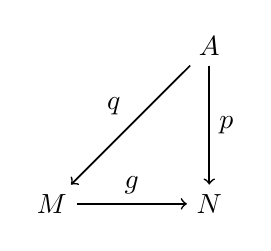
\begin{tikzpicture}[->,-latex, auto, main path/.style={->, semithick}, main node/.style={}]
\node	[main node]		(1) at (0,0)		{$M$};
\node	[main node]		(2) at (2,0)		{$N$};
\node [main node]		(3) at (2,2)		{$A$};

\draw (1) edge [main path] node [auto] {$g$} (2);
\draw (3) edge [main path] node [auto] {$p$} (2);
\draw (3) edge [main path] node [auto, swap] {$q$} (1);
\end{tikzpicture}
\end{equation*}
\end{mydef}

\begin{mydef}
A module $P$ is \emph{projective} if, whenever $g:M\to N$ is surjective and $p:P\to N$ is any map, there exists a lifting $q:P \to M$ making the following diagram commutes:
\begin{equation*}
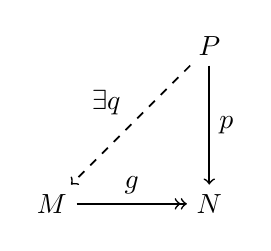
\begin{tikzpicture}[->,-latex, auto, main path/.style={->, semithick}, main node/.style={}]
\node	[main node]		(1) at (0,0)		{$M$};
\node	[main node]		(2) at (2,0)		{$N$};
\node [main node]		(3) at (2,2)		{$P$};

\draw (1) edge [->>, semithick] node [auto] {$g$} (2);
\draw (3) edge [main path] node [auto] {$p$} (2);
\draw (3) edge [dashed, ->, semithick] node [auto, swap] {$\exists q$} (1);
\end{tikzpicture}
\end{equation*}
\end{mydef}

\begin{prop} \label{projectiveprop}
The following for a module $P$ are equivalent:
\begin{description}
\item [(i)] P is projective.
\item [(ii)] The sequence $0\xrightarrow{}Hom(P, L)\xrightarrow{}Hom(P, M)\xrightarrow{}Hom(P, N)\xrightarrow{}0$ is exact for any short exact sequence $0\xrightarrow{}L\xrightarrow{}M\xrightarrow{}N\xrightarrow{}0$.
\item [(iii)]Any short exact sequence $0\xrightarrow{}L\xrightarrow{}M\xrightarrow{}P\xrightarrow{}0$ splits.
\item [(iv)]$P$ is isomorphic to a direct summand of free modules.
\end{description}
\end{prop}
\begin{proof} (i) $\Rightarrow$ (ii): As $P$ is projective we have that,
\begin{equation*}
\begin{tikzpicture}[->,-latex, auto, main path/.style={->, semithick}, main node/.style={}]
\node	[main node]		(1) at (0,0)		{$M$};
\node	[main node]		(2) at (2,0)		{$N$};
\node [main node]		(3) at (2,2)		{$P$};
\node [main node]		(4) at (-2, 0)		{$L$};
\node [main node]		(5) at (-4, 0)		{$0$};
\node [main node]		(6) at (4, 0)		{$0$};

\draw (1) edge [->>, semithick] node [auto] {$g$} (2);
\draw (3) edge [main path] node [auto] {$p$} (2);
\draw (3) edge [dashed, ->, semithick] node [auto, swap] {$\exists q$} (1);
\draw (4) edge [main path] node [auto] {$f$} (1);
\draw (5) edge [main path] (4);
\draw (2) edge [main path] (6);
\end{tikzpicture}
\end{equation*}
Hence, we have $q\in Hom(P,M)$ such that $gq=p\in Hom(P,N)$ which can also we written $p=gq=g_{\ast}(q)\in im(g_{\ast})$, defining a surjective map, $g_{\ast}: Hom(P,M) \to Hom(P,N)$. Thus,
\begin{equation*}
0\xrightarrow{}Hom(P,L) \xrightarrow{}Hom(P,M)\xrightarrow{g_{\ast}}Hom(P,N)\xrightarrow{}0
\end{equation*}
is exact by Proposition \ref{exactpropertiesprop}.\\
(ii) $\Rightarrow$ (iii): By assumption, if we have the short exact sequence $0\xrightarrow{}L\xrightarrow{}M\xrightarrow{}P\xrightarrow{}0$ then we have an exact sequence,
\begin{equation*}
0\xrightarrow{}Hom(P,L) \xrightarrow{}Hom(P,M)\xrightarrow{}Hom(P,P)\xrightarrow{}0.
\end{equation*}
Then we can lift the identity map $id_P\in Hom(P,P)$ to some $q\in Hom(P,M)$, such that:
\begin{equation*}
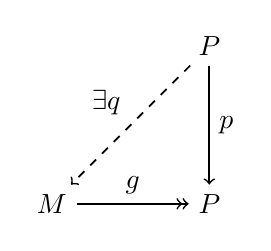
\begin{tikzpicture}[->,-latex, auto, main path/.style={->, semithick}, main node/.style={}]
\node	[main node]		(1) at (0,0)		{$M$};
\node	[main node]		(2) at (2,0)		{$P$};
\node [main node]		(3) at (2,2)		{$P$};

\draw (1) edge [->>, semithick] node [auto] {$g$} (2);
\draw (3) edge [main path] node [auto] {$p$} (2);
\draw (3) edge [dashed, ->, semithick] node [auto, swap] {$\exists q$} (1);
\end{tikzpicture}
\end{equation*}
Thus $g:M\to P$ is a retraction as we have $q:P\to M$ such that $gq=id_P$. Hence, $0\xrightarrow{}L\xrightarrow{}M\xrightarrow{}P\xrightarrow{}0$ splits by Lemma \ref{splittinglem}.\\
(iii)$\Rightarrow$ (iv): By choosing a generating set of $P$ we get a surjection from a free module $F$ onto $P$, $g:F\to P$, and this gives the short exact sequence, 
\begin{equation*}
0\xrightarrow{}ker(g)\xrightarrow{}F\xrightarrow{g}P\xrightarrow{}0,
\end{equation*}
and this splits by assumption. Hence, $F\cong ker(g)\oplus P$ and so $P$ is a direct summand of $F$ by Corollary \ref{MLNcor}.\\
(iv) $\Rightarrow$ (i): By assumption, $P$ is a direct summand of $F$ and so there are maps $r: F \to P$ and $s: P \to F$ with $rs=id_P$. Now consider the diagram, 
\begin{equation*}
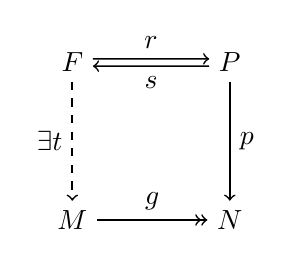
\begin{tikzpicture}[->,-latex, auto, main path/.style={->, semithick}, main node/.style={}]
\node	[main node]		(1) at (0,0)		{$M$};
\node	[main node]		(2) at (2,0)		{$N$};
\node [main node]		(3) at (2,2)		{$P$};
\node [main node]		(4) at (0,2)		{$F$};

\draw (1) edge [->>, semithick] node [auto] {$g$} (2);
\draw (3) edge [main path] node [auto] {$p$} (2);
\draw (4) edge [dashed, ->, semithick] node [auto, swap] {$\exists t$} (1);
\path (4.10) edge [main path] node [auto] {$r$} (3.170);
\path (3.190) edge [main path] node [auto] {$s$} (4.-10);
\end{tikzpicture}
\end{equation*}
where $g$ is surjective. The composite map $pr: F \to N$; since $F$ is free, it is surjective, and so there is a map $t: F \to M$ with $gt=pr$. Define $q: P \to M$ by $q=ts$ and then we can see that $gq=p$ as,
\begin{equation*}
gq=gts=prs=pid_P=p.
\end{equation*}
Hence $P$ is projective.
\end{proof}

As with projective modules we will use the first property given in \cite{CB1} to define injective modules, and then provide the properties as in \cite{CB1} with some details from \cite{Rotman}.

\begin{mydef}
A module $I$ is \emph{injective} if, whenever $f: L \to M$ is an injection, there exists a map $j: M \to I$ which extends any map $i: M \to I$, making the following diagram commute.
\begin{equation*}
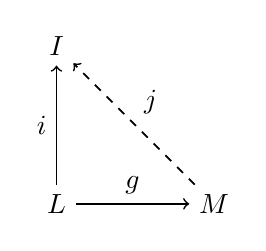
\begin{tikzpicture}[->,-latex, auto, main path/.style={->, semithick}, main node/.style={}]
\node	[main node]		(1) at (0,0)		{$L$};
\node	[main node]		(2) at (2,0)		{$M$};
\node [main node]		(3) at (0,2)		{$I$};

\draw (1) edge [main path] node [auto] {$g$} (2);
\draw (1) edge [main path] node [auto] {$i$} (3);
\draw (2) edge [dashed, ->, semithick] node [auto, swap] {$j$} (3);
\end{tikzpicture}
\end{equation*}
\end{mydef}

\begin{prop}
The following properties of a module $I$ are equivalent:
\begin{description}
\item [(i)] $I$ is injective.
\item [(ii)] The sequence $0\xrightarrow{} Hom(N, I) \xrightarrow{} Hom(M, I) \xrightarrow{} Hom(L, I) \xrightarrow{} 0$ is exact for any short exact sequence $0\xrightarrow{} L \xrightarrow{} M\xrightarrow{} N \xrightarrow {} 0$.
\item [(iii)] Any short exact sequence $0 \xrightarrow{} I \xrightarrow{} M \xrightarrow{} N \xrightarrow{}0$ splits.
\end{description}
\end{prop}
\begin{proof}
(i) $\Rightarrow$ (ii) $\Rightarrow$ (iii): Dual to Proposition \ref{projectiveprop}  for projectives.
(iii) $\Rightarrow$ (i): Consider the $0\xrightarrow{}L\xrightarrow{}M\xrightarrow{}\sfrac{M}{L} \xrightarrow{} 0$ and construct it's pushout along $\theta: L \to I$:
\begin{equation*}
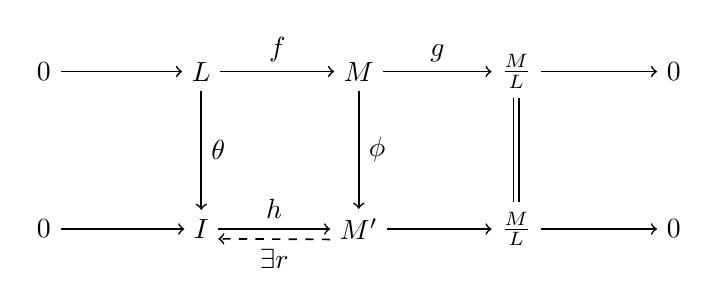
\begin{tikzpicture}[->,-latex, auto, main path/.style={->, semithick}, main node/.style={}]

\node	[main node]		(2) at (2,0)		{$0$};
\node	[main node]		(3) at (4,0)		{$L$};
\node [main node]		(4) at (6,0)		{$M$};
\node [main node]		(5) at (8,0)		{$\frac{M}{L}$};
\node	[main node]		(11) at (10,0)	{$0$};

\node	[main node]		(7) at (2,-2)		{$0$};
\node	[main node]		(8) at (4,-2)		{$I$};
\node [main node]		(9) at (6,-2)		{$M'$};
\node [main node]		(10) at (8,-2)	{$\frac{M}{L}$};
\node [main node]		(13) at (10,-2)	{$0$};

\draw (2) edge [main path] node [auto] {$$} (3);
\draw (3) edge [main path] node [auto] {$f$} (4);
\draw (4) edge [main path] node [auto] {$g$} (5);
\draw (5) edge [main path] (11);

\draw (7) edge [main path] node [auto] {$$} (8);
\path (8.0) edge [main path] node [auto] {$h$} (9.180);
\path (9.200) edge [dashed, ->, semithick] node [auto] {$\exists r$} (8.330);
\draw (9) edge [main path] node [auto, swap] {$$} (10);
\draw (10) edge [main path] (13);

\draw (3) edge [main path] node [auto] {$\theta$} (8);
\draw (4) edge [main path] node [auto] {$\phi$} (9);
\draw (5) edge [-, semithick, double, double distance=1.5pt](10);
\end{tikzpicture}
\end{equation*}
By assumption $0\xrightarrow{}I\xrightarrow{}M'\xrightarrow{}\sfrac{M}{L}\xrightarrow{}0$ splits and so $h:I \to M'$ has a retraction $r:M'\to I$. Then,
\begin{equation*}
r\phi f=rh\theta=\theta,
\end{equation*}
so $r\phi : M \to I$ extends $\theta: L \to I$. Hence $I$ is injective.
\end{proof}










\chapter{Representation of Quivers}

%%%%%%%%%%%%%%%%%%%%%%%%%%%%%%%%%%%%%%%%%%%%%%%%%%%%%%
%%%%%%%%%%%%%%		Quivers and Path Algebras	%%%%%%%%%%%%%%%%%%%%%%%
%%%%%%%%%%%%%%%%%%%%%%%%%%%%%%%%%%%%%%%%%%%%%%%%%%%%%%%

\section{Quivers and Path Algebras}

\begin{mydef}
A \emph{quiver} is defined as the tuple of sets and functions, $\mathbf{Q}=(Q_0\text{, }Q_1\text{, }s\text{, }t: Q_1 \to Q_0)$ such that:
\begin{itemize}
\item $Q_0$ is the set of vertices, which we will set to be the finite set $\{1, 2, \dots, n\}$.
\item $Q_1$ is the set of arrows, which we will also set to be finite.
\item Functions $s, t$ such that an arrow $\rho \in Q_1$ \emph{starts} at the vertex $s(\rho)\in Q_0$ and \emph{terminates} at the vertex $t(\rho)\in Q_0$, i.e. $\rho: s(\rho) \to t(\rho)$.
\end{itemize}
\end{mydef}

\begin{eg} \label{ininquivereg}
A quiver $Q=(Q_0, Q_1, s, t:Q_1 \to Q_0)$ where $Q_0=\{1, 2, 3, 4\}$, $Q_1=\{\alpha, \beta\}$, and $s, t$ are defined such that;
\begin{align*}
s:& Q_1 \to Q_0\text{,\quad} \alpha \mapsto 1\text{, } \beta \mapsto 2\text{, } \gamma \mapsto 4\\
t:& Q_1 \to Q_0\text{,\quad} \alpha \mapsto 2\text{, } \beta \mapsto 3\text{, } \gamma \mapsto 3,
\end{align*}
looks like,
\equ
\mathbf{Q}: \qquad
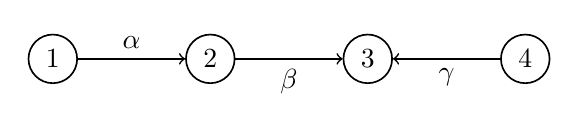
\begin{tikzpicture}[->,-latex, auto, every path/.style={->, semithick}, main node/.style={draw, circle}]
\node	[main node]		(1) at (0,0)		{1};
\node	[main node]		(2) at (2,0)		{2};
\node	[main node]		(3) at (4,0)		{3};
\node [main node]		(4) at (6,0)		{4};

\draw (1) edge node [auto] {$\alpha$} (2);
\draw (2) edge node [auto, swap] {$\beta$} (3);
\draw (4) edge node [auto] {$\gamma$} (3);
\end{tikzpicture}
\eequ
\end{eg}

\begin{mydef}
A \emph{non-trivial path}, $p$, in a quiver is a sequence of arrows $\rho_1, \dots, \rho_n$ which satisfies $t(\rho_{i+1})=s(\rho_i)$ for all $1\leq i <n$, i.e. the start of an arrow is where the previous arrow terminated. The starting and terminatinating vertex of a path $p$ are denoted $s(p)$ and $t(p)$, respectively.
\end{mydef}

\begin{note}
In this report the arrows in a path will be ordered the same way as the composition of functions, as in \cite{CB2}, however, be aware that other publications may order the arrows the opposite way.
\end{note}

\begin{mydef}
The \emph{trivial path} is the path which contains no arrows, i.e. it is a single vertex, and is denoted $e_i$ where the vertex is $i$.
\end{mydef}

\begin{eg} \label{ininpatheg}
The paths of the quiver in Example \ref{ininquivereg} are:
\equ
p_1=e_1, \quad p_2=e_2, \quad p_3=e_3, \quad p_4=e_4, \quad p_5=\alpha, \quad p_6=\beta, \quad p_7=\gamma, \quad p_8=\beta\alpha.
\eequ
However, $\gamma\beta\alpha$ is not a path because $t(\gamma)=3\neq s(\beta)=2$.
\end{eg}

\begin{mydef}
A \emph{path algebra} $kQ$ is the $k$-alegbra which has the basis all the paths in $Q$, and the product of two paths $p,q$ is defined as,
\equ
pq=\begin{cases}
\text{obvious composition} & \text{if } t(q)=s(p),\\
0 & \text{otherwise.}
\end{cases}
\eequ
This multiplication is assosciative.
\end{mydef}

\begin{eg}
If we once again use the quiver $Q$ from Example \ref{ininquivereg}, then, from Example \ref{ininpatheg}, we know the basis of the path algebra $kQ$ will be,
\equ
\{e_1, e_2, e_3, e_4,\alpha, \beta, \gamma, \beta\alpha\}.
\eequ
The product of $\beta$ and $\alpha$ is $\beta\alpha$, but the product of $\alpha$ and $\beta$ is zero, and the product of $e_2$ and $\alpha$ is just $\alpha$.
\end{eg}

\begin{eg}
If $Q$ is the following quiver,
\equ
\mathbf{Q}: \qquad
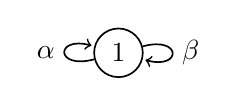
\begin{tikzpicture}[->,-latex, auto, every path/.style={->, semithick}, main node/.style={draw, circle}]
\node	[main node]		(1) at (0,0)		{1};

\draw (1) edge[loop left] node [auto] {$\alpha$} (1);
\draw (1) edge [loop right] node [auto] {$\beta$} (1);
\end{tikzpicture}
\eequ
forms the path algebra $kQ\cong k[X, Y]$, the free, assosciative algebra on two letters. In fact, if we have a quiver with a single vertex and $n$ loops, then this can be associated with the free, assosciated algebra on $n$ letters.
\end{eg}

\begin{eg} \label{UTpathalgebraeg}
If we have the quiver,
\equ
\mathbf{Q}: \qquad
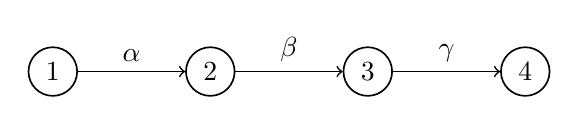
\begin{tikzpicture}[->,-latex, auto, every path/.style={->, semithick}, main node/.style={draw, circle}]
\node	[main node]		(1) at (0,0)		{1};
\node [main node]		(2) at (2,0)		{2};
\node [main node]		(3) at (4,0)		{3};
\node [main node]		(4) at (6,0)		{4};

\draw (1) edge node [auto] {$\alpha$} (2);
\draw (2) edge node [auto] {$\beta$} (3);
\draw (3) edge node [auto] {$\gamma$} (4);
\end{tikzpicture}
\eequ
the the path algebra, $kQ \cong UT_4(k)$ by the isomorphism,
\begin{multline*}
\lambda_1e_1+\lambda_2e_2+\lambda_3e_3+\lambda_4e_4+\lambda_5\alpha+\\
\lambda_6\beta+\lambda_7\gamma+\lambda_8\beta\alpha+\lambda_9\gamma\beta\alpha+\lambda_{10}\gamma\beta
\mapsto
\begin{pmatrix*}
\lambda_4 & \lambda_7 & \lambda_{10} & \lambda_9 \\
0 & \lambda_3 & \lambda_6 & \lambda_{8}\\
0 & 0 & \lambda_2 & \lambda_5 \\
0 & 0 & 0 & \lambda_1
\end{pmatrix*}
\end{multline*}
Generally, a quiver of the form,
\equ
\mathbf{Q'}: \qquad
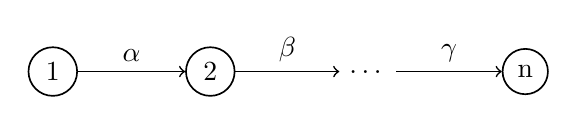
\begin{tikzpicture}[->,-latex, auto, every path/.style={->, semithick}, main node/.style={draw, circle}]
\node	[main node]		(1) at (0,0)		{1};
\node [main node]		(2) at (2,0)		{2};
\node []			(3) at (4,0)		{$\dots$};
\node [main node]		(4) at (6,0)		{n};

\draw (1) edge node [auto] {$\alpha$} (2);
\draw (2) edge node [auto] {$\beta$} (3);
\draw (3) edge node [auto] {$\gamma$} (4);
\end{tikzpicture}
\eequ
induces a path alegbra $kQ' \cong UT_n(k)$ for any $n$.
\end{eg}

\begin{eg}
In fact, we find that if $Q$ is the same quiver as above in Example \ref{UTpathalgebraeg}, then $kQ \cong LT_4(k)$ as well, through the isomorphism,
\begin{multline*}
\lambda_1e_1+\lambda_2e_2+\lambda_3e_3+\lambda_4e_4+\lambda_5\alpha+\\
\lambda_6\beta+\lambda_7\gamma+\lambda_8\beta\alpha+\lambda_9\gamma\beta\alpha+\lambda_{10}\gamma\beta
\mapsto
\begin{pmatrix*}
\lambda_1 & 0 & 0 & 0\\
\lambda_5 & \lambda_2 & 0 & 0\\
\lambda_8 & \lambda_6 & \lambda_3 & 0\\
\lambda_9 & \lambda_{10} & \lambda_7 & \lambda_4
\end{pmatrix*}.
\end{multline*}
Once again, this extends to the general case that, $kQ' \cong LT_n(k)$.
\end{eg}

\begin{eg} \label{pathalgebramatrixeg}
In a more general case, as long as there is only one path between any two vertices, we can identify $kQ$ with the following subalgebra of $M_n(k)$,
\equ
\{M \in M_n(k): M_ij=0 \text{ if there is no path from } j \text{ to }i\}.
\eequ
For instance, if we have the quiver,
\equ
\mathbf{Q}: \qquad
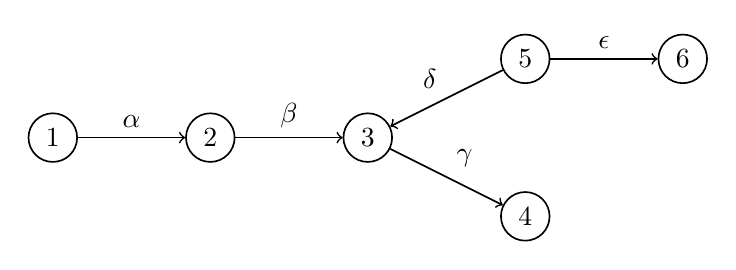
\begin{tikzpicture}[->,-latex, auto, every path/.style={->, semithick}, main node/.style={draw, circle}]
\node	[main node]		(1) at (0,0)		{1};
\node [main node]		(2) at (2,0)		{2};
\node [main node]		(3) at (4,0)		{3};
\node [main node]		(4) at (6,-1)		{4};
\node [main node]		(5) at (6,1)		{5};
\node [main node]		(6) at (8, 1)		{6};

\draw (1) edge node [auto] {$\alpha$} (2);
\draw (2) edge node [auto] {$\beta$} (3);
\draw (3) edge node [auto] {$\gamma$} (4);
\draw (5) edge node [auto, swap] {$\delta$} (3);
\draw (5) edge node [auto] {$\epsilon$} (6);
\end{tikzpicture}
\eequ
the we can see that the path algebra $kQ$ is isomorphic to the subalgebra with matrices of the form,
\equ
\begin{pmatrix*}
1 & 0 & 0 & 0 & 0 & 0 \\
1 & 1 & 0 & 0 & 0 & 0 \\
1 & 1 & 1 & 0 & 1 & 0 \\
1 & 1 & 1 & 1 & 1 & 0 \\
0 & 0 & 0 & 0 & 1 & 0 \\
0 & 0 & 0 & 0 & 1 & 1
\end{pmatrix*}
\eequ
\end{eg}

\begin{rem}
Note that the idea here has some parallels to similar results for directed graphs in graph theory.
\end{rem}

The following results about the idempotents of path alegebras are from \cite{CB2}, however, we have either given a proof or expanded upon the one given. For the following results we set $A=kQ$ and the $e_i$ are the trivial paths of $Q$.

\begin{lem} 
The $e_i$ are orthogonal, idempotents in $A$, i.e. $e_ie_i=e_i$ and $e_ie_j=0$ where $i\neq j$. Thus $\sum_{i=1}^{n}{e_i}=1_{A}$.
\end{lem}
\begin{proof}
Well, obviously, $e_ie_j=0$ when$i\neq j$ because $t(e_j)\neq s(e_i)$ because they are the trivial paths at different vertices, $i$ and $j$. Similarly, if we have the product $e_ie_i$ then the composition makes sense here because $t(e_i)=s(e_i)$, but the composition is just $e_i$ becuase if we travel along the trivial path $e_i$ twice, then this is just the same as travelling the trivial path. \\
If we have some path $p$ of the quiver, then bear in mind that,
\equ
e_ip=
\begin{cases}
e_ip=p & \text{if } i=t(p),\\
0 & \text{otherwise.}
\end{cases}
\eequ
Hence, the sum of the trivial paths acting on our path $p$ becomes, 
\equ
\big(\sum^{n}_{i=1}{e_i}\big)p=(e_1+e_2+\dots +e_n)p=e_ip=p=1_Ap,
\eequ
because only one of the $e_i$ in the sum will satisfy $i=t(p)$ and all the rest will give zero. Similary, we can show that $p\big(\sum^{n}_{i=1}{e_i}\big)=p1_A$.
\end{proof}

\begin{lem} \label{idempotentspaceslem}
The bases of the spaces $Ae_i$ and $e_jA$ are all the paths starting at $i$ and all the paths terminating at $j$, respectively. It then follows that the space $e_jAe_i$ has as a basis the paths that start at $i$ and terminate at $j$.
\end{lem}
\begin{proof}
For some $i\in Q_0$, and $A$ has the basis $\{p_1, p_2, \dots, p_n\}$, then as $Ae_i$ is a subspace of $A$ the basis of $Ae_i$ must be a subset of the basis of $A$, so, 
\equ
Ae_i=\{ae_i:a\in A\}=span\{p_1e_i+p_2e_i+\dots+p_ne_i\},
\eequ
and we know that,
\equ
p_re_i=
\begin{cases}
p_r & \text{if } s(p_r)=i,\\
0 & \text{otherwise}.
\end{cases}
\eequ
Hence, we can see that the basis of $Ae_i$ must be all the paths starting at $i$. Similarly, as $e_jA$ is a subspace of $A$ snd so following a similar argument we can see that its basis must be all the paths terminating at $j$. The result for $e_jAe_i$ follows from these as it simply the intersection of the two spaces.
\end{proof}

\begin{lem}
$A=\oplus^n_{i=1}Ae_i$, so each $Ae_i$ is a projective left $A$-module.
\end{lem}
\begin{proof}
From Lemma \ref{idempotentspaceslem} we know that for each $i$, the basis of $Ae_i$ are all the paths starting at $i$ and so $\oplus^n_{i=1}Ae_i$ must have as a basis all the paths starting at every vertex in $Q$, hence all the paths in $Q$. Thus $A=\oplus^n_{i=1}Ae_i$. Also, each $Ae_i$ is obviously a left $A$-module with the action defined as multiplication by $e_i$. Hence, each $Ae_i$ is a projective, left $A$-module.
\end{proof}

\begin{rem}
Similarly, $A=\oplus_{i=1}^ne_jA$, so each $e_jA$ is a projective, right $A$-module.
\end{rem}

\begin{lem} \label{idempotenthomlem}
If $X$ is a left $A$-module, then $Hom_A(Ae_i,X)\cong e_iX$.
\end{lem}
\begin{proof}
Well, we want to show that there are some maps $f$ and $g$ such that they satisfy,
\equ
Hom_A(Ae_i, X) \xleftrightarrow[g]{f}e_iX
% How to get two separate arrows here?
\eequ
Well, first consider the map $\theta: Ae_i \to X$ and so $\theta \in Hom_A(Ae_i, X)$, then we can have $f$ such that $f(\theta)=\theta(e_i)=\theta(e_i^2)=e_i\theta(e_i)\in e_iX$. Hence, $f$ maps a homomorphism from $Hom_A(Ae_i, X)$ to an element in $e_iX$.  Now consider the map $g(x): Ae_i \to X$, $g(x)(a)=ax$. We can check this is an $A$-module homomorphism as, 
\begin{align*}
g(x)(a+b) &=(a+b)x=ax+bx=g(x)(a)+g(x)(b)\text{ } & a, b\in Ae_i,\\
g(x)(\lambda a) &=\lambda a x=\lambda g(x)(a) \text{ } & \lambda\in A, a \in Ae_i.
\end{align*}
Hence, $g \in Hom_A(Ae_i, X)$. However, we can also have that $g: eX \to Hom_A(Ae_i, X)$ through $x \mapsto g(x)(r)$. \\
So now we need to show that $f$ and $g$ are inverse contructions of one another. We have for some $\theta \in Hom_A(Ae_i, X)$, 
\begin{align*}
\theta \xrightarrow{f} & \theta(e_i)\\
g(\theta(e_i))(a)=a\theta(e_i)=\theta(ae_i) \xleftarrow[g]{} & \theta(e_i)
\end{align*}
but $a\in Ae_i$ and so $a=\lambda e_i$ for some $\lambda\in A$, hence $ae_i=\lambda e_i^2=\lambda e_i=a$. Thus, $g(\theta(e_i))(a)=\theta(ae_i)=\theta(a)$ so $g(\theta(e_i))=\theta$ and $f$ and $g$ are inverses.
\end{proof}

\begin{lem} \label{idempotent0lem}
If $0\neq a \in Ae_i$ and $0\neq b\in e_iA$ then $ab\neq 0$.
\end{lem}
\begin{proof}
We know that $a$ and $b$ must have the forms, $a=\lambda_1p_1+ \dots \lambda_np_n$ and $b=\mu_1q_1 + \dots \mu_mq_m$ where the $p$ are paths starting at vertex $i$, the $q$ are paths termination at vertex $i$ and $p_r, q_r$ are paths of length $r$. Then the longest path in the product $ab$ must be $\lambda_n\mu_mp_nq_m$ and so $\lambda_n\mu_m \neq 0$ and $p_nq_m \neq 0$, so the product $ab\neq 0$.
\end{proof}

\begin{lem}
The $e_i$ are primitive idempotents, i.e. $Ae_i$ is an indecomposable module.
\end{lem}
\begin{proof}
From Lemma \ref{idempotenthomlem} we know that $End_A(Ae_i) \cong e_iAe_i$ and if this contains an idempotent $\epsilon$, then $\epsilon^2=\epsilon=\epsilon e_i$, so $\epsilon(e_i- \epsilon)=0$, but from Lemma \ref{idempotent0lem} we know that this can not happen if $\epsilon, (e_i-\epsilon) \neq 0$, thus we must have that either $\epsilon=0$ or $\epsilon=e_i$ and the result follows.
\end{proof}

\begin{lem} \label{idempotentsi=jlem}
If $e_i \in Ae_jA$ then $i=j$.
\end{lem}
\begin{proof}
For similar reasoning as in Lemma \ref{idempotentspacelem}, we can see that $Ae_jA$ has as a basis all the paths in $A$ which pass through the vertex $j$ and, by the definition of the trivial path, $e_i$ cannot pass through the vertex $j$ unless $i=j$ and so if $e_i \in Ae_jA$ we must have that $i=j$.
\end{proof}

\begin{lem}
The $e_i$ are inequivalent, i.e. $Ae_i \not\cong Ae_j$ for $i \neq j$.
\end{lem}
\begin{proof}
Two idempotent elements $e_i, e_j$ are said to be equivalent iff there exists some $u\in e_iAe_j$ and $v \in e_jAe_i$ such that $uv=e_i$ and $vu=e_j$. From Lemma \ref{idempotenthomlem} we can see that $Hom(Ae_i, Ae_j)\cong e_iAe_j$ and $Hom(Ae_j, Ae_i)\cong e_jAe_i$, and so inverse isomorphisms give elements $u$ and $v$ as described above with $uv=e_i$ and $vu=e_j$. However, this means that the path $e_i$ must pass through the vertex $j$ at some point, and vice versa, which contradicts Lemma \label{idempotenti=jlem}.
\end{proof}

\begin{eg}
Consider the quiver from Example \ref{pathalgebramatrixeg}, 
\equ
\mathbf{Q}: \qquad
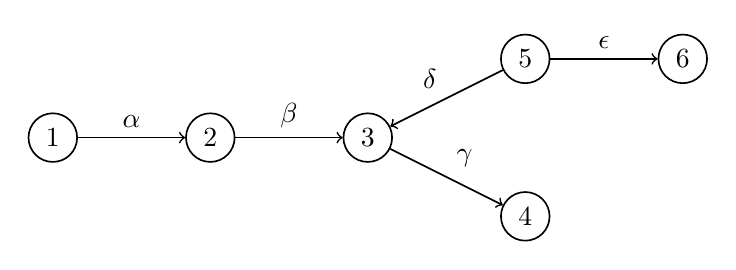
\begin{tikzpicture}[->,-latex, auto, every path/.style={->, semithick}, main node/.style={draw, circle}]
\node	[main node]		(1) at (0,0)		{1};
\node [main node]		(2) at (2,0)		{2};
\node [main node]		(3) at (4,0)		{3};
\node [main node]		(4) at (6,-1)		{4};
\node [main node]		(5) at (6,1)		{5};
\node [main node]		(6) at (8, 1)		{6};

\draw (1) edge node [auto] {$\alpha$} (2);
\draw (2) edge node [auto] {$\beta$} (3);
\draw (3) edge node [auto] {$\gamma$} (4);
\draw (5) edge node [auto, swap] {$\delta$} (3);
\draw (5) edge node [auto] {$\epsilon$} (6);
\end{tikzpicture}
\eequ
then we have have the following examples displaying the previous results for the idempotents of $kQ$. Let $A=kQ$.
\begin{enumerate}
\item We can see that $e_1e_1=e_1$ and $e_1e_2=0$. Also, $1_{A}=e_1 + e_2 + e_3 +e_4+e_5+e_6$ and so
\begin{align*}
1_A\gamma\beta&=(e_1 + e_2 + e_3 +e_4+e_5+e_6)\gamma\beta, \\
&=e_1\gamma\beta + e_2\gamma\beta + e_3\gamma\beta + e_4\gamma\beta + e_5\gamma\beta +e_6 \gamma\beta,\\
&=e_4\gamma\beta,\\
&=\gamma\beta.
\end{align*}
\item Now we can see that $Ae_1$ is spanned by all the paths starting at vertex 1, as,
\begin{align*}
Ae_1&=\{ae_1: a \in A\},\\
&=span_k\{\sum pe_1: p \text{ is in the basis of }A\},\\
&=span_k\{e_1e_1 + e_2e_1 + e_3e_1 +e_4e_1+e_5e_1+e_6e_1+\alpha e_1 + \\
&\qquad \qquad  \beta e_1 + \gamma e_1 + \delta e_1 +\epsilon e_1 +\beta\alpha e_1 + \gamma\beta e_1 + \gamma\delta e_1 + \gamma\beta\alpha e_1\}, \\
&=span_k\{e_1 + \alpha + \beta\alpha + \gamma\beta\alpha\}, \\
&=span_k\{\text{all paths starting at vertex 1}\}.
\end{align*}
Similarly, we can see that,
\begin{align*}
e_3A&=\{e_3a: a\in A\},\\
&=span_k\{e_3+\beta+\delta+\beta\alpha\},\\
&=span_k\{ \text{all the paths terminating at vertex 3}\}.
\end{align*}
Then we can see that, 
\begin{align*}
e_3Ae_1&=\{e_3ae_1: a \in A\},\\
&= span_k\{\beta\alpha\},\\
&=span_k\{\text{all paths starting at vertex 1 and terminating at vertex 3}\}.
\end{align*}
\item We can see that, 
\begin{align*}
\oplus^6_{i=1}Ae_i&=Ae_1 \oplus Ae_2 \oplus Ae_3 \oplus Ae_4 \oplus e_5 \oplus e_6, \\
&=span_k\{e_1 + \alpha + \beta\alpha + \gamma\beta\alpha\} \oplus span_k\{e_2 + \beta +\gamma\beta\} \oplus span_k\{e_3 + \gamma\} \oplus span_k\{e_4\} \oplus span_k\{e_5 + \delta + \epsilon + \gamma\delta\} + span_k\{e_6\}, \\
&= A.
\end{align*}
\end{enumerate}
\end{eg}

The following properties of path algebras are from \cite{CB2}, where they are given as exercises. In this report we will present them with proofs. Once again $A=kQ$.

\begin{lem}
$A$ is finite dimensional if and only if $Q$ has no oriented cycles.
\end{lem}
\begin{proof}
$\Rightarrow:$ If $Q$ has an oriented cycle then it will have a infinite number of paths as you can keep going round the cycle. This means that the basis of $A$, which is all the paths in $Q$, will be infinite, and so $A$ will not be finite dimensional.\\
$\Leftarrow:$ If $Q$ has no oriented cycles then it must have a finite number of paths and so the basis of $A$ will be finite and hence $A$ will be finite dimensional.
\end{proof}

\begin{eg}
If we consider the quiver $Q$, 
\equ
\mathbf{Q}: \qquad
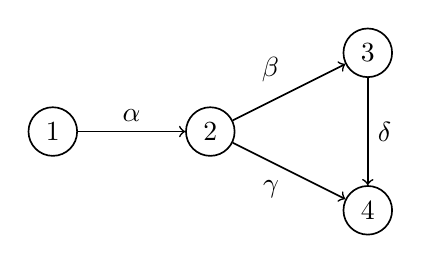
\begin{tikzpicture}[->,-latex, auto, every path/.style={->, semithick}, main node/.style={draw, circle}]
\node	[main node]		(1) at (0,0)		{1};
\node [main node]		(2) at (2,0)		{2};
\node [main node]		(3) at (4,1)		{3};
\node [main node]		(4) at (4,-1)		{4};

\draw (1) edge node [auto] {$\alpha$} (2);
\draw (2) edge node [auto] {$\beta$} (3);
\draw (2) edge node [auto, swap] {$\gamma$} (4);
\draw (3) edge node [auto] {$\delta$} (4);
\end{tikzpicture}
\eequ
and we can see that $Q$ has the paths $e_1, e_2, e_3, e_4, \alpha, \beta, \gamma, \delta, \beta\alpha, \gamma\alpha, \beta\delta, \delta\beta\alpha$, and so the basis of $A$ is $\{e_1, e_2, e_3, e_4, \alpha, \beta, \gamma, \delta, \beta\alpha, \gamma\alpha, \beta\delta, \delta\beta\alpha\}$, which is finite, and so $A$ is finite dimensional. \\
However, if we have the quiver $Q'$, 
\equ
\mathbf{Q'}: \qquad
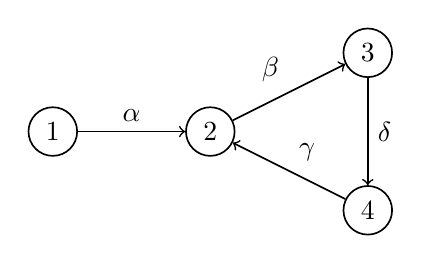
\begin{tikzpicture}[->,-latex, auto, every path/.style={->, semithick}, main node/.style={draw, circle}]
\node	[main node]		(1) at (0,0)		{1};
\node [main node]		(2) at (2,0)		{2};
\node [main node]		(3) at (4,1)		{3};
\node [main node]		(4) at (4,-1)		{4};

\draw (1) edge node [auto] {$\alpha$} (2);
\draw (2) edge node [auto] {$\beta$} (3);
\draw (4) edge node [auto, swap] {$\gamma$} (2);
\draw (3) edge node [auto] {$\delta$} (4);
\end{tikzpicture}
\eequ
it has paths $e_1, e_2, e_3, e_4, \alpha, \beta, \gamma, \delta, \beta\alpha,\delta\beta, \gamma\delta, \delta\beta\alpha, \gamma\delta\beta\alpha, \beta\gamma\delta\beta\alpha, \delta\beta\gamma\delta\beta\alpha, \dots$, and so on, an infinte number of paths, meaning that the basis of $A$ is infinte and hence $A$ is not finite dimensional.
\end{eg}

\begin{lem}
$A$ is prime, i.e. $IJ\neq 0$ for two sided ideals $I, J \neq 0$ if and only if for all $i, j \in Q_0$ there exists a path $i$ to $j$.
\end{lem}
\begin{proof}
\emph{Need to include proof here}
\end{proof}

\begin{lem}
$A$ is left noetherian if and only if, if there is an oriented cycle through the vertex $i$, then only one arrow starts at the vertex $i$.
\end{lem}
\begin{proof}
Let $Ap$ represent the left-ideal whose basis are all the paths starting with $p$ for any path $p$. \\
Suppose we have a quiver $Q$ of the form,
\equ
\mathbf{Q}: \qquad
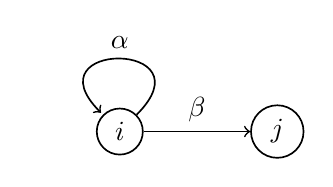
\begin{tikzpicture}[->,-latex, auto, every path/.style={->, semithick}, main node/.style={draw, circle}]
\node	[main node]		(1) at (0,0)		{$i$};
\node [main node]		(2) at (2,0)		{$j$};

\draw (1) edge [loop] node [auto, swap] {$\alpha$} (1);
\draw (1) edge node [auto] {$\beta$} (2);
\end{tikzpicture}
\eequ
assuming $i\neq j$ and where $\alpha$ represents an orientated cycle, then we can see that,
\equ
A\beta+A\beta\alpha+\dots +A\beta\alpha^n \subseteq A\beta+A\beta\alpha+\dots +A\beta\alpha^{n+1}.
\eequ
However, since $e_j\beta\alpha^{n+1}\not \in A\beta+A\beta\alpha+\dots +A\beta\alpha^n$ the inclusion is strict. Hence, if $Q$ is of the form above, there is an ascending chain of left ideals, 
\equ
A\beta \subset A\beta + A\beta\alpha \subset A\beta + A\beta\alpha+A\beta\alpha^2 \subset \dots
\eequ
which does not terminate and so $A$ is not noetherian.\\
Suppose that for all $i\in Q_0$, if $\alpha$ an oriented cycle where $s(\alpha)=i$, then for all $\rho \in Q_1$, $\rho=\alpha_1$ or $s(\rho)\neq i$; where $\alpha=\alpha_1\alpha_2\dots\alpha_m$ for some $\alpha_1, \dots, \alpha_m \in Q_1$. This means there are some $\rho_1, \dots, \rho_n$ paths such that given any path $\beta\in A$ we have that $\beta=q\rho_j$ for some $j\in\{1, \dots, n\}$ and some $q$ a path in an oriented cycle.
Now if we let $Q'$ be the quiver, and  $A'$ the corresponding path algebra, where, 
\equ
Q'_0=Q_0\text{ \& } Q_1=Q'_1\cup \{a\in Q_1: a \text{ is not in an oriented cycle of }Q\}.
\eequ
So, for any basis element $\beta$ of $A$, $\beta=qp_j$ where $q$ is a path in $A'$. Following the previous two results we can see that, 
\begin{equation}
A=A'\rho_1+A'\rho_2 + \dots +A'p_n
\end{equation}
\begin{claim}
 If $S$ is a subring of a ring $R$ and $R$ is finitely generated as a left $S$-module, then, if $S$ is a noetherian ring, so is $R$.
\end{claim}
\begin{proof}
From the result that a finitely generated module over a noetherian ring is noetherian, gives us that $R$ is noetherian as a left $S$-module. Let $I_1 \subseteq I_2 \subseteq \dots$ be an ascending chain of left ideals in $R$, and each $I_k$ is a left $S$-submodule of $R$; so by the above, this chain terminates.
\end{proof}
Using the above Claim and the earlier result that $A$ is finitely generated as a left $A'$-module, we can see that our problem of proving that $A$ is left noetherian reduces to proving that $A'$ is left noetherian.\\
Now let $\alpha^{(l)}_j$ be the $j^{th}$ arrow of the $l^{th}$ oriented cycle in $Q'$ and then, 
\equ
Q'_1=\{\alpha^{(l)}_j : j \in \{1, \dots, q_l\}, l \in \{1, \dots, r\}\}.
\eequ
Consider the endomorphism, 
\begin{align*}
X_l: &A' \to A', \\
&e_t(p) \mapsto \alpha^{(l)}_{k-1}\alpha^{(l)}_{k-2}\dots \alpha^{(l)}_{1}\alpha^{(l)}_{q_l}\dots \alpha^{(l)}_{k}p\text{, where } t(p)=t=s(\alpha^{(l)}_{k}), \\
&\text{otherwise }\mapsto 0.
\end{align*}
We can adapt Hilbert's Basis Theorem to show that $k[X_1, \dots, X_r]$ is a noetherian ring and we can see that $A'$ is a finitely generated $k[X_1, \dots, X_r]$-module. Hence, $A'$ is left noetherian, and so $A$ is left noetherian.
\end{proof}

\begin{mydef}
We can define the \emph{length} of any path $p$ by the following: Let, 
\equ 
length(p)=length(\sum_{\text{arrows }\rho}\lambda_{\rho}\rho):=max\{length(\rho):\lambda_\rho\neq0\},
\eequ
where $\lambda_\rho\neq 0$ for some $\rho$. 
\end{mydef}

\begin{lem}
The basis of $J(A)$ is $\{\text{path } i \text{ to }j: \text{ there is no path from } j \text{ to }i\}$.
\end{lem}
\begin{proof}
Firstly, lets prove that, 
\equ
J'(A):= span_k\{\text{paths }p:s(p)=i, t(p)=j\text{with no paths from $j$ to $i$}\}\subseteq J(A).
\eequ
Given any $w\in J'(A)$ we have that, 
\begin{enumerate}
\item $(wp)^2=0$ for any path $p$.
\begin{proof}
There are no paths $p$ such that $t(p)=s(w)$ and $s(p)=t(w)$, so $wpw=0$, so $wpwp=(wp)^2=0$.
\end{proof}
\item $(w(p+p'))^2=0$ for any path $p$ and $\lambda\in k$.
\begin{proof}
\equ
(w(p+p'))^2=(wp+wp')^2=(wp)^2+wpwp'+wp'wp +(wp')^2
\eequ
As $wpw$ and $wp'w$ are both equal to zero by the above, we have that, $(w(p+p'))^2=0$.
\end{proof}
\item $(w(\lambda p))^2=\lambda^2(wp)^2=0$
\begin{proof}
By item 1.
\end{proof}
\end{enumerate}
Now let $w\in J'(A)$ and $z\in A$, then,
\equ
wz=u\big(\sum_{\text{paths }p}\lambda_pp\big)=w\big(\sum_{\substack{\text{paths }p:\\t(p)=s(w)}}\lambda_pp\big):=\tau
\eequ
and from above we can see that $\tau^2=0$, meaning $(wz)^2=0$, so, $(1+wz)(1-wz)=1$, hence, $1+wz\in U(A)$ for all $z\in A$. Thus $w\in J(A)$.\\
Now we want to prove that $J(A)\subseteq J'(A)$. Let $w$ be a basis element of $J(A)$ coming from the basis of $A$. Suppose also that $length(w)=0$, so $w=e_i$ for some $i\in Q_0$. Let, 
\equ
M_i:=\sum_{\substack{\text{paths }p:\\ p\neq e_i}}Ap,
\eequ
then $M_i\unlhd A$ and if $M_i\subsetneq N \unlhd A$, then, $e_i\in N$, so, $N=A$; hence, $M_i$ is a maximal left ideal, but $w\not \in M_i$ contradicting that $w \in J(A)$.Hence, $length(w)>0$.\\
Now suppose $w\not \in J'(A)$, so there's a path $p$ such that $s(w)=t(p)$ and $s(p)=t(w)$. Since $w \in J(A)$ and $p\in A$,  $1+wp \in U(A)$, so there exists some $z\in A$ such that $(1+wp)z=1$, with, 
\equ
z=\sum^m_{l=0}\sum_{\substack{\text{paths }p: \\ length(p_l)=l}}\lambda_{p_l}p_l.
\eequ
Since, $length(1)=length(l_1+\dots+l_n)=0$, we have that, 
\begin{align*}
0&=length((1+wp)z),\\
&=length(z+wpz),\\
&=max(length(z), length(wpz)),
\end{align*}
so $wpz=0$ as otherwise $length(wpz)=0$, contradicting that $length(w)>0$. So as $(1+wp)z=z+wpz=1$, $z=1$, so $wp=0$, a contradiction.
\end{proof}

\begin{lem}
The centre of $A$ is $k\times k\times \dots k[T] \times k[T] \times \dots$, with one factor for each connected component $C$ of $Q$, and that the factor is $k[T]$ if and only if $C$ is an oriented cycle.
\end{lem}
\begin{proof}
Firstly, we know that if our quiver $Q$ is composed of $n$ connected components $C_1, \dots, C_n$ then we our path algebra looks like $kQ=kC_1 \times kC_2 \times \dots \times kC_n$.
\begin{claim}
Where $Z(A)$ represents the centre of $A$, we have that, 
\equ
Z(A\times B)=Z(A) \times Z(B).
\eequ
\end{claim}
\begin{proof}
Suppose we have $(a, b)\in Z(A \times B)$, then we have that,
\begin{align*}
& (a, b)(a', b')=(a', b')(a, b) \forall (a',b')\in A\times B,\\
\Leftrightarrow &(aa',bb')=(a'a,b'b) \forall a'\in A, b' \in B, \\
\Leftrightarrow & aa'=a'a \text{ \& } bb'=b'b \forall a'\in A, b'\in B,\\
\Leftrightarrow & a\in Z(A) \text{ \& } b\in Z(B).
\end{align*}
Hence, $Z(A \times B)\cong Z(A) \times Z(B)$.
\end{proof}
Now, using the claim, we can see that,
\equ
Z(kQ) \cong Z(kC_1) \times Z(kC_2) \times \dots \times Z(kC_n),
\eequ
Now, assume the connected component $C_i$ is not an oriented cycle, and consider $a\in Z(kC_i)$, which is a linear combination of paths. Let us choose a path of maximal length $\rho_1\dots \rho_m$, and say there exists some $\sigma$ such that we can have $\sigma \rho_1 \dots \rho_m$ but with $t(\sigma)\neq s(\rho_m)$, but since $\rho_1 \dots \rho_m$ was maximal this path is involved $\sigma a=a\sigma$ as $a\in Z(A)$. So, $a \sigma$ is also a linear combination of paths, i.e. $\tau_1 \dots \tau_m\sigma$, wheere $\tau_1\dots\tau_m$ is a path in $a$.This causes, 
\equ
\sigma\rho_1\dots\rho_m=\tau_1\dots\tau_m\sigma,
\eequ
which implies that $\sigma=\rho_m$, which causes an oriented cycle, hence a contradiction. Thus, $Z(kC_i)\cong k$.\\
\emph{Need to complete the case for oriented cycle connected component.}

\end{proof}

\begin{eg}
Consider the quiver, 
\equ
\mathbf{Q}: \qquad
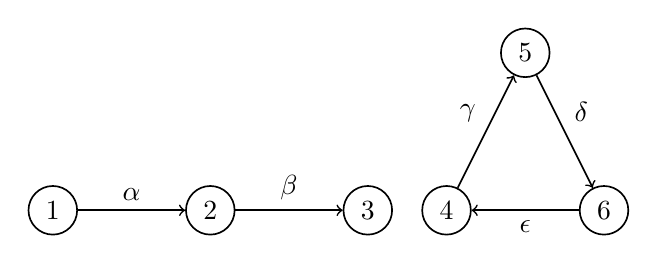
\begin{tikzpicture}[->,-latex, auto, every path/.style={->, semithick}, main node/.style={draw, circle}]
\node	[main node]		(1) at (0,0)		{1};
\node [main node]		(2) at (2,0)		{2};
\node [main node]		(3) at (4,0)		{3};
\node [main node]		(4) at (5,0)		{4};
\node [main node]		(5) at (6,2)		{5};
\node [main node]		(6) at (7, 0)		{6};

\draw (1) edge node [auto] {$\alpha$} (2);
\draw (2) edge node [auto] {$\beta$} (3);
\draw (4) edge node [auto] {$\gamma$} (5);
\draw (5) edge node [auto] {$\delta$} (6);
\draw (6) edge node [auto] {$\epsilon$} (4);
\end{tikzpicture}
\eequ
and so, $Z(kQ)=Z(kC_1) \times Z(kC_2)$, where $C_2$ is the oriented cycle component. Then, 
\begin{align*}
Z(kC_1)=&\{a \in kC_1: ac=ca \forall c\in kC_1\}, \\
&=\{\lambda(e_1+e_2+e_3): \lambda\in k\}, \\
&\cong k,
\end{align*}
since none of the elements of $kC_1$ are commutative, apart from the identity. Also, 
\begin{align*}
Z(kC_2) &=\{a \in kC_2: ac=ca \forall c\in kC_2\},\\
&=\{\lambda(\gamma\delta\epsilon + \delta\epsilon\gamma +\epsilon\gamma\delta): \lambda \in k\}, \\
&\cong k[T], \text{ where }T=\gamma\delta\epsilon + \delta\epsilon\gamma +\epsilon\gamma\delta, 
\end{align*}
because none of the elements of $kC_2$ are commutative other than the identity element. Thus, $Z(kQ)\cong k \times k[T]$.
\end{eg}

%%%%%%%%%%%%%%%%%%%%%%%%%%%%%%%%%%%%%%%%%%%%%%%%%%%%%%%
%%%%%%%%%%%		Representations of Quivers	%%%%%%%%%%%%%%%%%%%%%%%%%%
%%%%%%%%%%%%%%%%%%%%%%%%%%%%%%%%%%%%%%%%%%%%%%%%%%%%%%%

\section{Representations of Quivers}

\begin{mydef}
A \emph{representation} $X$ of a quiver $Q$ is given by considering each vertex $i\in Q_0$ as a vector space $X_i$, and each arrow $\rho \in Q_1$ as a linear map $X_\rho: X_{s(\rho)} \to X_{t(\rho)}$.
\end{mydef}

\begin{eg}
Let $Q$ be the quiver, 
\equ
\mathbf{Q}: \qquad
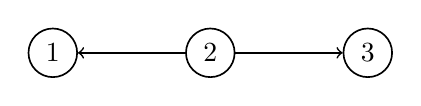
\begin{tikzpicture}[->,-latex, auto, every path/.style={->, semithick}, main node/.style={draw, circle}]
\node	[main node]		(1) at (0,0)		{1};
\node [main node]		(2) at (2,0)		{2};
\node [main node]		(3) at (4,0)		{3};

\draw (2) edge (1);
\draw (2) edge (3);
\end{tikzpicture}
\eequ
then we can have representations $X$ and $Y$, 
\equ
\mathbf{X}: \quad
\begin{tikzpicture}[->,-latex, auto, every path/.style={->, semithick}, main node/.style={draw, circle}]
\node	[]		(1) at (0,0)		{$k$};
\node []		(2) at (2,0)		{$k$};
\node []		(3) at (4,0)		{$k$};

\draw (2) edge node [auto, swap] {$\alpha$} node [auto] {1} (1);
\draw (2) edge node [auto] {$\beta$} node [auto, swap] {1} (3);
\end{tikzpicture}
\qquad \& \qquad
\mathbf{Y}: \quad
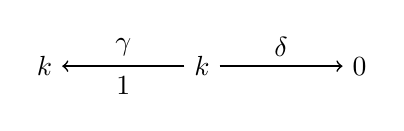
\begin{tikzpicture}[->,-latex, auto, every path/.style={->, semithick}, main node/.style={draw, circle}]
\node	[]		(1) at (0,0)		{$k$};
\node []		(2) at (2,0)		{$k$};
\node []		(3) at (4,0)		{$0$};

\draw (2) edge node [auto, swap] {$\gamma$} node [auto] {1} (1);
\draw (2) edge node [auto] {$\delta$} (3);
\end{tikzpicture}
\eequ
\end{eg}

\begin{mydef}
A \emph{morphism} $\theta: X \to X'$ between representationsis given by linear maps $\theta_i:X_i \to X'_i$ for each $i\in Q_0$ satisfy $X'_{\rho}\theta _{s(\rho)} = \theta_{t(\rho)}X_{\rho}$ for each $\rho \in Q_1$. The \emph{composition} of morphisms, $\theta: X \to X'$ with $\phi: X' \to X''$ is given by $(\phi \theta)_i=\phi_i \theta_i$.
\end{mydef}

\begin{eg}
\end{eg}





\section{Standard Resolution}

\section{Bricks}

\section{Dynkin and Euclidean diagrams}


\chapter{Auslander-Reiten Quivers}














\begin{thebibliography}{99}

\bibitem{CB1}
Crawley-Boevey, W.
\emph{Cohomology and Central Simple Algebras}. [Online-PDF file]. [Accessed October 2014].
Available from: http://www1.maths.leeds.ac.uk/~pmtwc/cohom.pdf.

\bibitem{CB2}
Crawley-Boevey, W.
\emph{Representation of Quivers}. [Online-PDF file]. [Accessed October 2014].
Available from: http://www1.maths.leeds.ac.uk/~pmtwc/quivlecs.pdf.

\bibitem{Rotman}
Rotman, J. J.
2009.
\emph{An Introduction to Homological Algebra}
2nd ed.
New York: Springer Science+Business Media.

\bibitem{Weibel}
Weibel, Charles A.
1995.
\emph{An Introduction to Homological Algebra}
Cambridge University Press

\bibitem{Stamm}
Hilton, P.J. \& Stammbach, U.
1972.
\emph{A Course in Homological Algebra}
1st ed.
Springer.

\bibitem{Schiff}
Schiffler, Ralf.
2014.
\emph{Quiver Representations}
Springer.

\bibitem{Splittinglem}
\emph{Splitting lemma - Wikipedia, the free encyclopedia.} [Online]  [Accessed 23 April 2015].
Available at: http://en.wikipedia.org/wiki/Splitting\_lemma.

\bibitem{Ext}
\emph{Ext functor - Wikipedia, the free encyclopedia.} [ONLINE]  [Accessed 29 April 2015].
Available at: http://en.wikipedia.org/wiki/Ext\_functor\#Ext\_and\_extensions.



\end{thebibliography}


\end{document}


\begin{equation*}
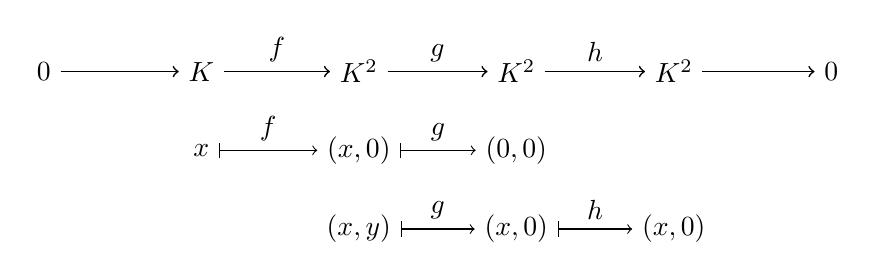
\begin{tikzpicture}[->,-latex, auto, main path/.style={->, semithick}, main node/.style={}]
\node [main node]		(1) at (0,0)		{$0$};
\node [main node]		(2) at (2,0)		{$K$};
\node [main node]		(3) at (4,0)		{$K^2$};
\node [main node]		(4) at (6,0)		{$K^2$};
\node [main node]		(5) at (8,0)		{$K^2$};
\node [main node]		(6) at (10,0)		{$0$};

\node[main node]		(7) at (2,-1)		{$x$};
\node[main node]		(8) at (4,-1)		{$(x,0)$};
\node [main node]		(9) at (6,-1)		{$(0,0)$};

\node [main node]		(10) at (4,-2)		{$(x,y)$};
\node [main node]		(11) at (6, -2)		{$(x, 0)$};
\node [main node]		(12) at (8, -2)		{$(x,0)$};

\draw (1) edge [main path] node [auto] {$$} (2);
\draw (2) edge [main path] node [auto] {$f$} (3);
\draw (3) edge [main path] node [auto] {$g$} (4);
\draw (4) edge [main path] node [auto] {$h$} (5);
\draw (5) edge [main path] node [auto] {$$} (6);

\draw [|->] (7) edge node [auto] {$f$} (8);
\draw [|->] (8) edge node [auto] {$g$} (9);

\draw [|->] (10) edge node [auto] {$g$} (11);
\draw [|->] (11) edge node [auto] {$h$} (12);
\end{tikzpicture}
\end{equation*}